%%%%%%%%%%%%%%%%%%%%%%%%%%%%%%%%%%%%%%%%%%%%%%%%%%%%%%%%%%%%%%%%%%%%%%%%%%%%
%DIF LATEXDIFF DIFFERENCE FILE
%DIF DEL ../R0/PW13Paper.tex   Wed Jan 25 16:56:32 2023
%DIF ADD ./PW13Paper.tex       Thu May 25 10:00:58 2023
% AGUJournalTemplate.tex: this template file is for articles formatted with LaTeX
%
% This file includes commands and instructions
% given in the order necessary to produce a final output that will
% satisfy AGU requirements, including customized APA reference formatting.
%
% You may copy this file and give it your
% article name, and enter your text.
%
%
% Step 1: Set the \documentclass
%
%

%% To submit your paper:
\documentclass[draft]{agujournal2019}
\usepackage{url} %this package should fix any errors with URLs in refs.
\usepackage{lineno}
%DIF 20a20
\usepackage[]{amssymb} %DIF > 
%DIF -------
% \graphicspath{{/Users/jklymak/Dropbox/PW13/satellite/doc/},
%               {/Users/jklymak/Dropbox/PW13/figs/mvp/},
%               {/Users/jklymak/Dropbox/PW13/analysis/mvp/doc/},
%               {/Users/jklymak/Dropbox/PW13/LaPerouse13/doc/},
%               {/Users/jklymak/Dropbox/PW13/auxdata/doc/}}

% \graphicspath{{./figs/}}
\DeclareGraphicsExtensions{%
              .pdf,.png}

%DIF 30d31
%DIF < 
%DIF -------
\usepackage[plain]{fancyref}
%DIF 32a32
\renewcommand*{\freffigname}{Fig.} %DIF > 
%DIF -------
% \usepackage[]{hyperref}
%\usepackage[inline]{trackchanges} %for better track changes. finalnew option will compile document with changes incorporated.
\usepackage{soul}
\linenumbers

\newcommand*{\Eddy}{{\sc Eddy}}
\draftfalse

\journalname{JGR: Oceans}
%DIF PREAMBLE EXTENSION ADDED BY LATEXDIFF
%DIF UNDERLINE PREAMBLE %DIF PREAMBLE
\RequirePackage[normalem]{ulem} %DIF PREAMBLE
\RequirePackage{color}\definecolor{RED}{rgb}{1,0,0}\definecolor{BLUE}{rgb}{0,0,1} %DIF PREAMBLE
\providecommand{\DIFadd}[1]{{\protect\color{blue}\uwave{#1}}} %DIF PREAMBLE
\providecommand{\DIFdel}[1]{{\protect\color{red}\sout{#1}}}                      %DIF PREAMBLE
%DIF SAFE PREAMBLE %DIF PREAMBLE
\providecommand{\DIFaddbegin}{} %DIF PREAMBLE
\providecommand{\DIFaddend}{} %DIF PREAMBLE
\providecommand{\DIFdelbegin}{} %DIF PREAMBLE
\providecommand{\DIFdelend}{} %DIF PREAMBLE
\providecommand{\DIFmodbegin}{} %DIF PREAMBLE
\providecommand{\DIFmodend}{} %DIF PREAMBLE
%DIF FLOATSAFE PREAMBLE %DIF PREAMBLE
\providecommand{\DIFaddFL}[1]{\DIFadd{#1}} %DIF PREAMBLE
\providecommand{\DIFdelFL}[1]{\DIFdel{#1}} %DIF PREAMBLE
\providecommand{\DIFaddbeginFL}{} %DIF PREAMBLE
\providecommand{\DIFaddendFL}{} %DIF PREAMBLE
\providecommand{\DIFdelbeginFL}{} %DIF PREAMBLE
\providecommand{\DIFdelendFL}{} %DIF PREAMBLE
%DIF COLORLISTINGS PREAMBLE %DIF PREAMBLE
\RequirePackage{listings} %DIF PREAMBLE
\RequirePackage{color} %DIF PREAMBLE
\lstdefinelanguage{DIFcode}{ %DIF PREAMBLE
%DIF DIFCODE_UNDERLINE %DIF PREAMBLE
  moredelim=[il][\color{red}\sout]{\%DIF\ <\ }, %DIF PREAMBLE
  moredelim=[il][\color{blue}\uwave]{\%DIF\ >\ } %DIF PREAMBLE
} %DIF PREAMBLE
\lstdefinestyle{DIFverbatimstyle}{ %DIF PREAMBLE
	language=DIFcode, %DIF PREAMBLE
	basicstyle=\ttfamily, %DIF PREAMBLE
	columns=fullflexible, %DIF PREAMBLE
	keepspaces=true %DIF PREAMBLE
} %DIF PREAMBLE
\lstnewenvironment{DIFverbatim}{\lstset{style=DIFverbatimstyle}}{} %DIF PREAMBLE
\lstnewenvironment{DIFverbatim*}{\lstset{style=DIFverbatimstyle,showspaces=true}}{} %DIF PREAMBLE
%DIF END PREAMBLE EXTENSION ADDED BY LATEXDIFF

\begin{document}

%% ------------------------------------------------------------------------ %%
%  Title
%
% (A title should be specific, informative, and brief. Use
% abbreviations only if they are defined in the abstract. Titles that
% start with general keywords then specific terms are optimized in
% searches)
%
%% ------------------------------------------------------------------------ %%

% Example: \title{This is a test title}

\title{Separation of an upwelling current bounding the Juan de Fuca Eddy}

%% ------------------------------------------------------------------------ %%
%
%  AUTHORS AND AFFILIATIONS
%
%% ------------------------------------------------------------------------ %%

% Authors are individuals who have significantly contributed to the
% research and preparation of the article. Group authors are allowed, if
% each author in the group is separately identified in an appendix.)

% List authors by first name or initial followed by last name and
% separated by commas. Use \affil{} to number affiliations, and
% \thanks{} for author notes.
% Additional author notes should be indicated with \thanks{} (for
% example, for current addresses).

% Example: \authors{A. B. Author\affil{1}\thanks{Current address, Antartica}, B. C. Author\affil{2,3}, and D. E.
% Author\affil{3,4}\thanks{Also funded by Monsanto.}}

\authors{Jody M.\ Klymak\affil{1,2}, Susan E.\ Allen\affil{3,4}, Stephanie Waterman\affil{3}}


\affiliation{1}{School of Earth and Ocean Sciences, University of Victoria, BC, Canada}
\affiliation{2}{Department of Physics \& Astronomy, University of Victoria, BC, Canada}
\affiliation{3}{Department of Earth, Ocean and Atmospheric Sciences, University of British Columbia, Vancouver, BC, Canada}
\affiliation{4}{Institute of Applied Mathematics, University of British Columbia, Vancouver, BC, Canada}
%(repeat as many times as is necessary)

%% Corresponding Author:
% Corresponding author mailing address and e-mail address:

\correspondingauthor{J.\ Klymak}{jklymak@uvic.ca}

%% Keypoints, final entry on title page.

%  List up to three key points (at least one is required)
%  Key Points summarize the main points and conclusions of the article
%  Each must be 140 characters or fewer with no special characters or punctuation and must be complete sentences

% Example:
% \begin{keypoints}
% \item	List up to three key points (at least one is required)
% \item	Key Points summarize the main points and conclusions of the article
% \item	Each must be 140 characters or fewer with no special characters or punctuation and must be complete sentences
% \end{keypoints}

\begin{keypoints}
\item The shelf break current along Vancouver Island separates downstream of a submarine bank.
\item Offshore water is drawn onto the shelf and forms a sharp semi-persistent front with the Juan de Fuca Eddy.
\item The Eddy shows evidence of long residence times, and little evidence of deep-water origin.
\end{keypoints}


\begin{abstract}

Observations of temperature, salinity, and oxygen on the southern Vancouver Island shelf show a large-scale exchange of shelf water with offshore water, just offshore of a semi-permanent recirculation\DIFdelbegin \DIFdel{.   The semi-permanent cyclonic recirculation (}\DIFdelend \DIFaddbegin \DIFadd{, often termed }\DIFaddend the Juan de Fuca Eddy\DIFdelbegin \DIFdel{) }\DIFdelend \DIFaddbegin \DIFadd{.   The Eddy }\DIFaddend occupies a region where the shelf widens abruptly in the lee of a bank.  The water in this Eddy is a mixture of offshore water and water from a buoyant coastal current.  This water is well-mixed along a mixing line in temperature-salinity space, though it retains stratification, and is either rapidly mixed or has a long residence time.  There is a \DIFdelbegin \DIFdel{sharp }\DIFdelend \DIFaddbegin \DIFadd{less than 1-km wide }\DIFaddend temperature-salinity front on the offshore side of this well-mixed water \DIFdelbegin \DIFdel{, no more than 1-km wide, and }\DIFdelend \DIFaddbegin \DIFadd{that }\DIFaddend has no sign of instabilities. The clearest evidence of cross-front transport is found during a \DIFdelbegin \DIFdel{short }\DIFdelend tidally resolved survey over a bank\DIFdelbegin \DIFdel{, and was }\DIFdelend \DIFaddbegin \DIFadd{. The transport is }\DIFaddend due to flows in the cross-bank direction \DIFdelbegin \DIFdel{driving large mixing in }\DIFdelend \DIFaddbegin \DIFadd{that also drive }\DIFaddend 50-m tall hydraulic jumps. Upstream of the \DIFdelbegin \DIFdel{recirculation }\DIFdelend \DIFaddbegin \DIFadd{Eddy }\DIFaddend there is an along-shelf current flowing equatorward.  However the whole current separates from the shelf before reaching the \DIFdelbegin \DIFdel{recirculation}\DIFdelend \DIFaddbegin \DIFadd{Eddy}\DIFaddend , in the lee of a bank, and is replaced by water from offshore.  The separation event was also seen in sea-surface temperatures from satellite images as a tongue of cool coastal water that is ejected offshore.

\end{abstract}

\section*{Plain Language Summary}

The southern Vancouver Island continental shelf is biologically productive due to high nutrient input from the Strait of Juan de Fuca and Salish Sea estuarine system and substantial cross-shelf transport due to the complicated topography.  Here we present intensive sampling of the Juan de Fuca Eddy region. The observations show that below the surface mixed layer, the water in the Eddy is low in oxygen, and has undergone substantial vertical and lateral mixing. In contrast to previous literature we find that the low oxygen in the \DIFdelbegin \DIFdel{eddy }\DIFdelend \DIFaddbegin \DIFadd{Eddy }\DIFaddend is likely because of respiration rather than being pulled from low-oxygen water in the California Undercurrent.

The observations also show a remarkable flow separation of the equatorward shelf current.  The current is seen to detach and is pushed offshore. Such events are readily seen in satellite imagery, but our observations indicate that the separation extends the depth of the water column on the shelf, and that this separation may be partially driven by the local bathymetry.  The separation is a very strong cross-shelf exchange event, and transports substantial nutrient-rich coastal water offshore to drive productivity in the deeper ocean adjacent to the continental slope.

%% ------------------------------------------------------------------------ %%
%
%  TEXT
%
%% ------------------------------------------------------------------------ %%


%%%%%%%%%%%%%%%%%%%%%%%%%%%%%%%%%%%%%%%%%%%%%%%%%%%%%%%%%%%%%%%%%%%%%
% MAIN BODY OF PAPER
%%%%%%%%%%%%%%%%%%%%%%%%%%%%%%%%%%%%%%%%%%%%%%%%%%%%%%%%%%%%%%%%%%%%%
\section{Introduction}

Cross-shelf exchange is important to the health and productivity of continental shelf regions, allowing for offshore oxygenated water to be exchanged with nutrient-rich, but oxygen-depleted, nearshore water.  Cross-shelf transport usually requires ageostrophic flow, since geostrophically balanced flow will tend to follow topographic contours, often providing a barrier to lateral exchange \cite{brink16}.  Mechanisms of cross-shelf exchange include internal waves and instabilities in shelf-break fronts.  However, these mechanisms can be smaller in magnitude compared to intermittent three-dimensional exchange, driven by eddying, often catalyzed by topographic irregularity \cite{barthetal00}.

Here we present detailed \emph{in-situ} observations from the southern Vancouver Island shelf, collected in summer 2013, and sampled by a rapid profiling vehicle equipped with a CTD and oxygen sensor, supplemented by traditional hydrographic surveys bracketing the high resolution observations by a month. The shelf has complicated bathymetry (\fref{fig:LocMapBoth}), with a relatively simple 50-km wide shelf poleward of our study site \DIFdelbegin \DIFdel{, }\DIFdelend that widens to over 75 km wide equatorward of La Perouse Bank.  The South Vancouver Island Shelf is this wide shelf region, characterized by a number of banks, and finally is incised on the \DIFdelbegin \DIFdel{poleward }\DIFdelend \DIFaddbegin \DIFadd{equatorward }\DIFaddend side by the Juan de Fuca \DIFdelbegin \DIFdel{canyon}\DIFdelend \DIFaddbegin \DIFadd{Canyon}\DIFaddend .   Water from the Strait of Juan de Fuca flows poleward as a buoyant current that hugs the coast \cite{thomsonetal89, hickeyetal91}, while shelf water flows equatorward in the summer both forced by local winds and via teleconnections with the long, homogenous shelves equatorward off Washington and Oregon \cite{hickeyetal91,thomsonkrassovski15,engidaetal16}.  Trapped between these two currents is a region of relatively homogenous water that has been termed the Juan de Fuca Eddy \cite{freelanddenman82,freelandmcintosh89,foremanetal07,macfadyenhickey10}, denoted ``\Eddy'' below.

A goal of our study was to understand how the \Eddy\ persists and how it exchanges water properties with offshore water.  We focus on water deeper than $50 \mathrm{m}$, below the summer mixed layer, because this water is trackable with water mass properties, even though the \Eddy\ is often studied from the point of view of the surface circulation \cite{macfadyenhickey10}.  Past studies \DIFdelbegin \DIFdel{have }\DIFdelend found low oxygen concentrations in the \Eddy, and inferred that water is upwelled from the California Undercurrent from as deep as 400 m \cite{freelanddenman82,deweycrawford88}.  This inference was based on the assumption that oxygen is \DIFdelbegin \DIFdel{conservative}\DIFdelend \DIFaddbegin \DIFadd{a conservative tracer}\DIFaddend , and hence water in the \Eddy\ had to come from  the oxygen minimum zone found further offshore \cite{mackasetal87}.  \DIFdelbegin \DIFdel{This lead to hypotheses that perhaps }\DIFdelend \DIFaddbegin \DIFadd{It was hypothesized that }\DIFaddend the \Eddy\ was fed by waters being drawn up a spur canyon (called the Spur Canyon) via ageostrophic transport from offshore to onshore due to low pressure in the \Eddy\ center \cite{weaverhsieh87}.  Below, we will argue that there is no evidence of such transport and that oxygen is likely low because of local consumption due to respiration.

A second goal of our study was to better understand cross-shore exchange between shelf and offshore water.  \DIFdelbegin \DIFdel{Cross-shore }\DIFdelend \DIFaddbegin \DIFadd{For a two-dimensional topography with along-shore wind forcing, cross-shore }\DIFaddend transport is supplied by Ekman layers\DIFdelbegin \DIFdel{in simple geometries under wind forcing}\DIFdelend . However, in many locations there is also evidence of eddies\DIFaddbegin \DIFadd{, meanders, }\DIFaddend and filaments driving wholesale separation of shelf currents into the deep ocean. \DIFaddbegin \DIFadd{These have been well-studied off California \mbox{%DIFAUXCMD
\cite{strubetal91} }\hskip0pt%DIFAUXCMD
where satellite and }\emph{\DIFadd{in-situ}} \DIFadd{observations show large meanders of coastal upwelling currents leading to coastal water injected into the offshore domain.   }\DIFaddend Along the Vancouver Island shelf, large \DIFdelbegin \DIFdel{filaments or }\DIFdelend instabilities of the coastal current have \DIFaddbegin \DIFadd{also }\DIFaddend been inferred using satellite images \cite{ikedaemery84,thomsongower98}.  Direct observations of such filaments have been made further to the south off Cape Blanco \cite{barthetal00}, and off other coasts \cite{relvasbarton05}. Net cross-shore transport of nutrients and chlorophyll have been found in hydrographic surveys off Vancouver Island \cite{mackasyelland99}, and associated with mesoscale features in geostrophic velocities and in satellite observations.  The mechanisms driving such separations are poorly understood, but hypotheses include coastal hydraulics leading to along-shore trapping of coastal waves \cite{dalebarth01},  wind stress curl variations \cite{castelaobarth07}, induced relative vorticity due to stretching of parcels that overshoot their initial isobaths due to a sudden change in downstream bathymetry \cite{dasaro88}, and, at this location, non-linear breaking of large-scale meanders due to baroclinic instability between the wind-driven current and the California Undercurrent \cite{ikedaetal84, batteen97}.

In this paper we present observations of water masses on the Southern Vancouver Island Shelf collected in 2013 (\fref{sec:Site}), presenting the data in a number of ways to highlight the important processes\DIFdelbegin \DIFdel{, with a }\DIFdelend \DIFaddbegin \DIFadd{.  We }\DIFaddend focus on the offshore side of the \Eddy\ region (\fref{sec:Observations}) where we consider the age of the \Eddy, the steadiness of the front separating the \Eddy\ and the offshore water, properties along the \DIFdelbegin \DIFdel{spur canyon }\DIFdelend \DIFaddbegin \DIFadd{Spur Canyon }\DIFaddend that was believed to feed the \Eddy, and a large offshore tongue of the shelf-break current and its intrusion into the interior.  We \DIFdelbegin \DIFdel{discuss }\DIFdelend \DIFaddbegin \DIFadd{conclude by discussing }\DIFaddend the origin of the \Eddy\ and the implications of the separating jet (\fref{sec:Summary}).

\section{Site and Methods}
\label{sec:Site}

\DIFdelbegin %DIFDELCMD < \begin{figure*}[htbp]
%DIFDELCMD <   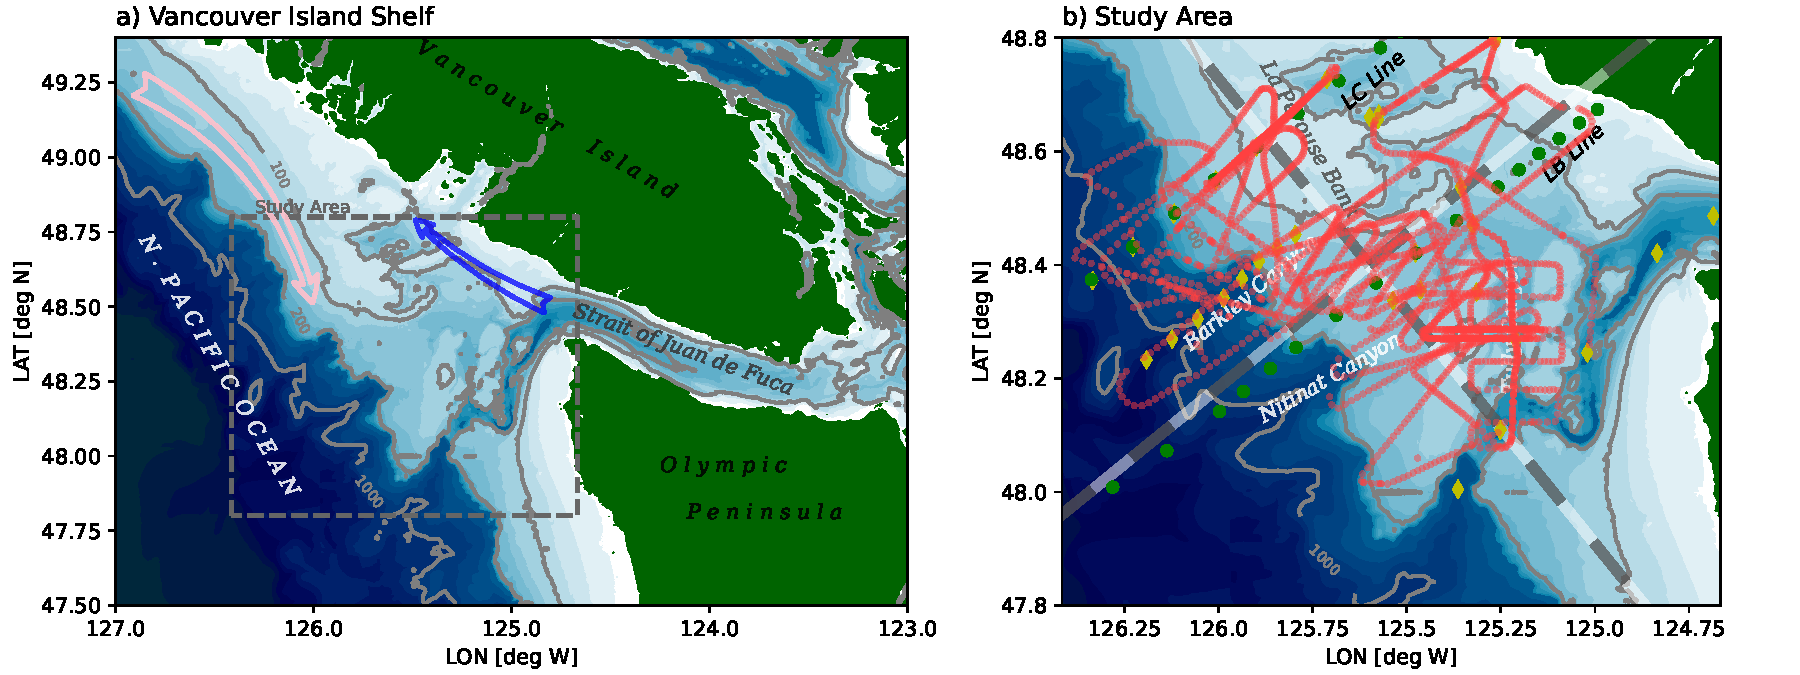
\includegraphics[width=5in]{LocMapBoth.pdf}
%DIFDELCMD <   %%%
\DIFdelendFL \DIFaddbeginFL \begin{figure}[htbp]
  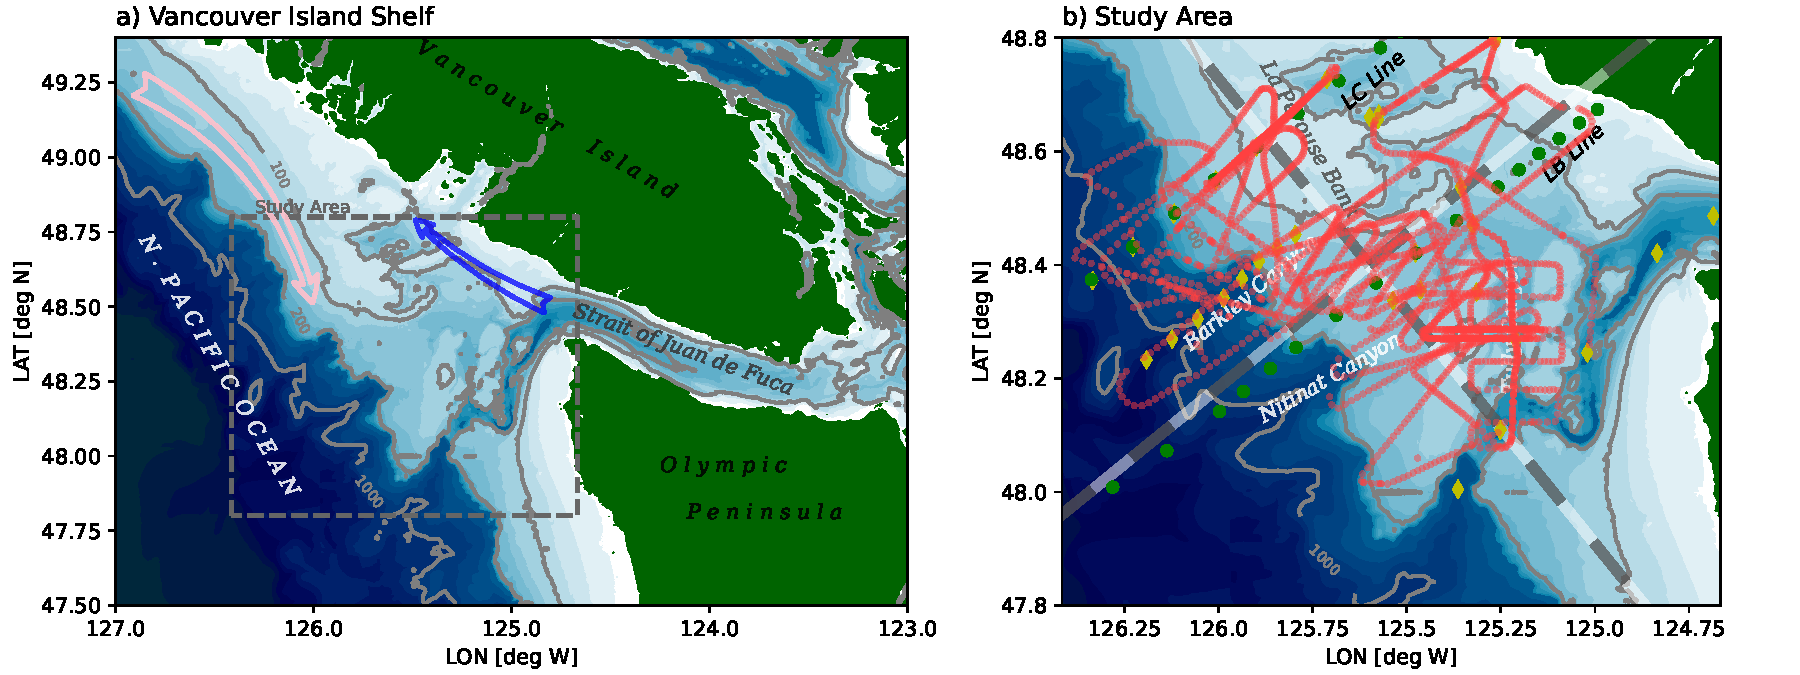
\includegraphics[width=5.4in]{LocMapBoth.pdf}
  \DIFaddendFL \caption{a) Study site on the Vancouver Island Shelf.  The blue arrow indicates the direction of the Vancouver Island Coastal Current, and the pink arrow indicates southward flow of the coastal upwelling current.  The dashed box indicates the approximate limits of the study area.  b) The study area with \DIFaddbeginFL \DIFaddFL{major bathymetric features labelled.  The coordinate system used for this paper is shown with alternating grey and white bands at 10-km intervals in the along- and cross-shore directions. c) sample locations with }\DIFaddendFL hydrographic casts from the La Perouse cruises along the LB and LC Lines (green dots), hydrographic casts during the Falkor cruise (yellow diamonds), and finescale Moving Vessel Profiler casts (red dots).  \DIFdelbeginFL \DIFdelFL{The coordinate system used for this paper }\DIFdelendFL \DIFaddbeginFL \DIFaddFL{Magenta
  square }\DIFaddendFL is \DIFdelbeginFL \DIFdelFL{shown with alternating grey and white bands at 10-km intervals in the along- and cross-shore directions}\DIFdelendFL \DIFaddbeginFL \DIFaddFL{La Perouse wind buoy}\DIFaddendFL .}
  \label{fig:LocMapBoth}
\DIFdelbeginFL %DIFDELCMD < \end{figure*}
%DIFDELCMD < %%%
\DIFdelend \DIFaddbegin \end{figure}
\DIFaddend 

The study site was the southern portion of the Vancouver Island Shelf (\fref{fig:LocMapBoth}a), a particularly complicated region due to the bathymetry and varied forcing.  At the south end of the study site is the Juan de Fuca \DIFdelbegin \DIFdel{canyon}\DIFdelend \DIFaddbegin \DIFadd{Canyon}\DIFaddend , which feeds dense water into Juan de Fuca Strait.  This dense water is mixed with fresh water from the Fraser River at the sills and archipelagos further inland and fluxes out the Strait again, where it turns poleward along Vancouver Island to form the Vancouver Island Coastal Current.  The Juan de Fuca Canyon has a notable spur canyon (Spur Canyon) \DIFdelbegin \DIFdel{, }\DIFdelend that incises the shelf towards the north into the study site (\fref{fig:LocMapBoth}b).  The rest of the shelf is punctuated by a series of banks and shallow basins.  La Perouse \DIFdelbegin \DIFdel{bank  }\DIFdelend \DIFaddbegin \DIFadd{Bank  }\DIFaddend separates the outer shelf from a deeper inner basin and forms the poleward boundary off where the shelf widens abruptly south of 48.5 N. Equatorward, the shelf widens further, and the shelf break has a series of submarine canyons, in particular Nitnat Canyon and Barkley Canyon.

We \DIFdelbegin \DIFdel{present observations }\DIFdelend \DIFaddbegin \DIFadd{use an along/across-shelf co-ordinate system with an origin at
48.4\textdegree N and 125.6\textdegree W, with the across-shelf $x$ oriented 39 degrees north of East (}\fref{fig:LocMapBoth}\DIFadd{b, grey/white alternating lines).  The projection is Cartesian with a central latitude at 48.4\textdegree N, which is sufficient for the limited geographic extents discussed here.
}

\DIFadd{Observations }\DIFaddend from La Perouse hydrographic surveys along the LB and LC lines, collected aboard the \emph{CCGS Tully} from 2013-05-30 to 2013-05-31  (``May''), and 2013-09-07 to 2013-09-09 (``September'') \DIFaddbegin \DIFadd{are used to put finescale observations in context of routine hydrographic work in the study region}\DIFaddend .  These lines span the 50 m isobath to deep offshore, with casts every $7.5\ \mathrm{km}$ across shelf. The data comes from a lowered Seabird 9-11 CTD, with an SBE 43 oxygen sensor.
\DIFdelbegin \DIFdel{Oxygen data have been corrected against bottle casts, and the CTD corrected for sensor offsets and thermal lags.
}\DIFdelend 

\DIFdelbegin \DIFdel{We focus }\DIFdelend \DIFaddbegin \DIFadd{The focus in this paper is }\DIFaddend on finescale surveys carried out between these hydrographic surveys, from 2013-08-21 to 2013-08-30.  Data were collected from the \emph{R/V Falkor} with an AML Oceanographic Moving Vessel Profiler (MVP).  Data was collected analogously to data collected during similar field campaigns \cite{klymaketal15a, klymaketal16, dasaroetal18}. The MVP was equipped with an AML Oceanographic CTD, and a Rinko Oxygen sensor with a 7-s response time foil.  The MVP profiled to depths of 200 m or to within 5 m of the seafloor, whichever was shallower, and dropped at a speed of approximately $3\ \mathrm{m\,s^{-1}}$.  Data collection took place while the ship cruised at speeds between 5 and 8 kts, usually at around 6 kts, to enable fine horizontal spacing of the casts, with typical spacing  of 800 m in deep water, and less in water shallower than 200 m.  Data is reported for the downcast, which mostly follows a vertical path.  The rapid speed of the profiling makes the oxygen measurements somewhat coarse, and probably biased due to the phase lag of the sensor, so we treat these qualitatively in this paper.

Unfortunately, neither vessel had an operational acoustic Doppler profiler during the cruises with which to make water velocity measurements.

Winds during the cruises were typical for the west coast of Vancouver Island, with equatorward upwelling-favorable winds during July and early August (\fref{fig:LaPeWind}).  During the finescale survey, and for the week previous, the winds were intermittently downwelling favorable.  Note that this locale is strongly affected by coastally trapped waves from further south, so doming of near-bottom isopycnals often persists despite local wind forcing, and takes a finite amount of time to spin down \cite{thomsonkrassovski15, engidaetal16}.

\begin{figure*}[htbp]
  \begin{center}
    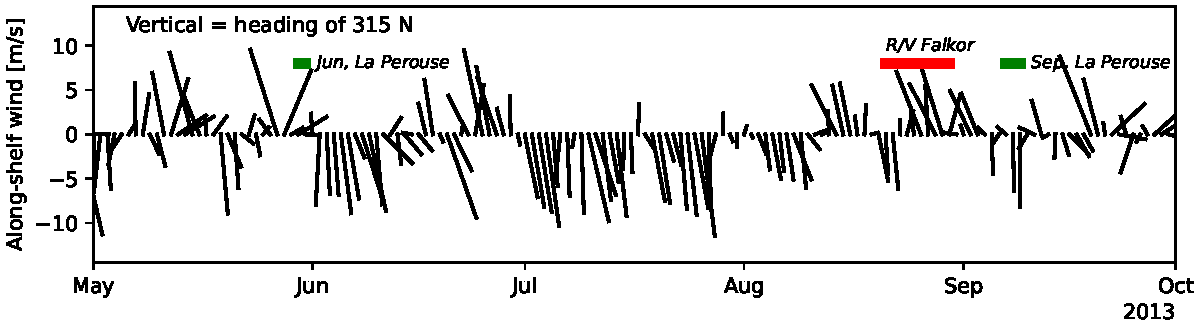
\includegraphics[width=5.5in]{LaPeWind}
    \caption{
      Wind from the La Perouse buoy \DIFaddbeginFL \DIFaddFL{at 48.84 N, 126 W }\DIFaddendFL \cite{DFOWind2013C46206}.  The vertical direction is along-shelf (chosen as a heading of 315 N), so vectors pointing straight down represent upwelling winds.  The wind components have been low-pass filtered to one-day averages.  The timing of the surveys discussed in the paper are shown as colored bands.
      \label{fig:LaPeWind} }
  \end{center}
\end{figure*}


\section{Observations}
\label{sec:Observations}

\subsection{Early and late summer hydrographic surveys}

Hydrographic sections along the LB and LC hydrographic lines highlight summer conditions on the Southern Vancouver Island Shelf and \DIFdelbegin \DIFdel{indicate some of the features we are focusing on in this paper }\DIFdelend \DIFaddbegin \DIFadd{are presented to give context to the more detailed survey carried out on the }\emph{\DIFadd{R/V Falkor}} \DIFaddend (\Fref{fig:LaPerouse2013Ctd}).  During both surveys, and along both lines, there is clear evidence of upwelling, with the $26.4\ \mathrm{kg\,m^{-3}}$ isopycnal reaching from 130 m depth offshore to shallower than 85 m over the shelf.  \DIFdelbegin \DIFdel{This }\DIFdelend \DIFaddbegin \DIFadd{The }\DIFaddend upwelled water tends to be low in oxygen and cool. Further onshore, the Vancouver Island Coastal Current hugs the coast, where isopycnals tilt down towards the shore,and water is warmer than offshore.

\begin{figure*}[htbp]
  \begin{center}
     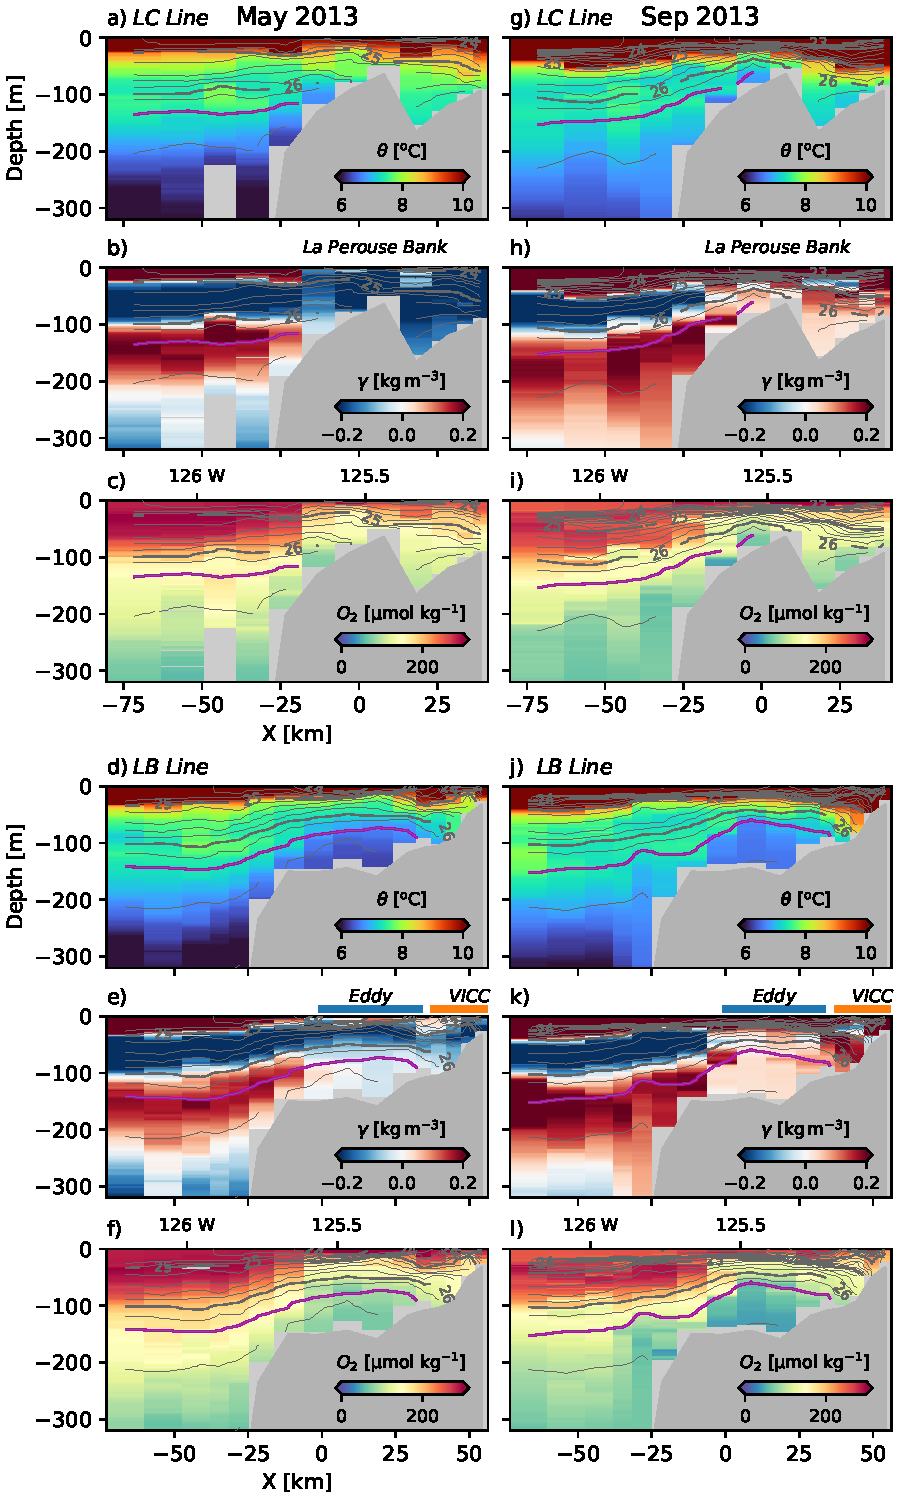
\includegraphics[width=5in]{LaPerouse2013Ctd}
     \caption{Observations along LC Line in May (a--c) and Sep (g--i) and LB lines in May (d--f) and Sep (j--l).  X is across-shelf distance in the coordinate system shown in \fref{fig:LocMapBoth}. Potential density is contoured every $0.2\ \mathrm{kg\,m^{-3}}$, with the $26.4\ \mathrm{kg\,m^{-3}}$ colored magenta.  Potential temperature, $\theta$, spice anomaly, $\gamma$ and oxygen concentration, $O_2$, are colored for each section.}
     \label{fig:LaPerouse2013Ctd}
  \end{center}
\end{figure*}

The Juan de Fuca Eddy region is observed along the LB Line (\fref{fig:LaPerouse2013Ctd}, bottom three rows), mostly inshore of 0 km. \DIFdelbegin \DIFdel{This water }\DIFdelend \DIFaddbegin \DIFadd{The water in the }\Eddy\DIFadd{\ }\DIFaddend is cooler and lower in oxygen than along the same isopycnal further offshore.  Near the surface, the isopycnals are domed, and the low-oxygen anomaly extends as high as the thin surface mixed layer.

The water upstream of the \Eddy\ region, along the LC line, is less mixed \DIFaddbegin \DIFadd{and has higher oxygen }\DIFaddend than the \Eddy\ water (\fref{fig:LaPerouse2013Ctd}, top three rows).  \DIFdelbegin \DIFdel{It does not show as much drawdown of oxygen, and is warmer, at least offshore of La Perouse bank ($X \approx 5\ \mathrm{km}$).  }\DIFdelend Based on these properties, offshore water does not appear to make it over La Perouse \DIFdelbegin \DIFdel{bank }\DIFdelend \DIFaddbegin \DIFadd{Bank }\DIFaddend into the onshore basin, or if it does, it does so intermittently and with substantial mixing. Note that the water along the $26.4\ \mathrm{kg\,m^{-3}}$ isopycnal \DIFaddbegin \DIFadd{(}\fref{fig:LaPerouse2013Ctd}\DIFadd{, magenta contours) }\DIFaddend becomes cooler and lower in oxygen where it intersects the shelf, consistent with both enhanced mixing near the shelf and with drawdown of oxygen by respiration.

The contrast in onshore and offshore waters can be clearly traced in temperature-salinity ($\theta$--$S$) anomalies along isopycnals (\fref{fig:LaPerouse2013TS}a).  Denser than $26.6\ \mathrm{kg\,m^{-3}}$, the deep water masses found offshore are largely homogenous. In the lighter water masses, there are distinct differences between warm and salty offshore water compared to water on the shelf at the same densities.

We use a spice anomaly defined as relative to a straight line in $\theta$--$S$
space (\fref{fig:LaPerouse2013TS}) representing an approximate mixing line for
water in the \Eddy, and passing through the points $7.75\ \mathrm{^oC}$, $30\
\mathrm{psu}$ and $6.6\ \mathrm{^oC}$, $35\ \mathrm{psu}$. Spice anomaly for a
given water sample at density $\sigma_{\theta}$ is given by $\gamma = \alpha
\left(T - T_0\left(\sigma_{\theta}\right)\right) + \beta \left(S -
S_0\left(\sigma_{\theta}\right)\right)$ where
$T_0\left(\sigma_{\theta}\right)$, where $S_0\left(\sigma_{\theta}\right)$ are
the temperature and salinity along the mixing line at the same density as the
water sample. The sign convention is that a positive anomaly is warmer and
saltier than data along the mixing line.

\begin{figure}[htbp]
  \begin{center}
     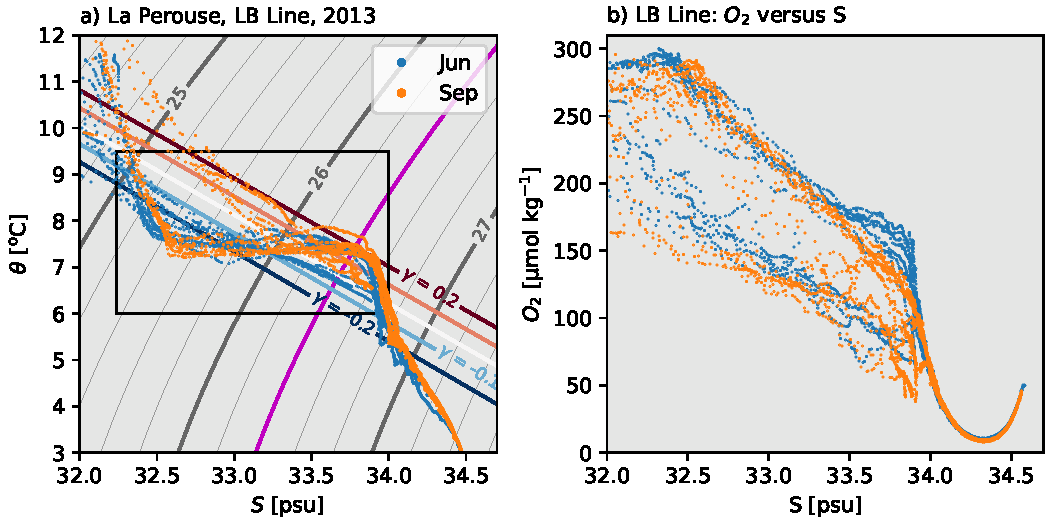
\includegraphics[width=5in]{LaPerouse2013TS}
     \caption{a) Potential temperature, $\theta$, versus salinity, $S$, for the La Perouse data shown in \fref{fig:LaPerouse2013Ctd}; potential density is contoured every $0.2\ \mathrm{kg\,m^{-3}}$, with the $26.4\ \mathrm{kg\,m^{-3}}$ colored magenta. A definition of spice anomaly is shown in this plot, and discussed in the text.  The rectangle is the $\theta-S$ range used in \fref{fig:TSdensSpice} below. b) The same data with oxygen concentration versus salinity.}
     \label{fig:LaPerouse2013TS}
  \end{center}
\end{figure}

Using this metric of spice anomaly, offshore water tends to have high absolute
values (\fref{fig:LaPerouse2013Ctd}, middle rows), with a positive-anomaly
layer (\DIFdelbegin \DIFdel{red}\DIFdelend \DIFaddbegin \DIFadd{$\gamma \approx 0.2\ \mathrm{kg\,m^{-3}}$, red colors}\DIFaddend ) centered at $26.4\
\mathrm{kg\,m^{-3}}$ sandwiched between negative-anomaly layers above and
below.  On the shelf ($-10\, \mathrm{km} < X < 30\, \mathrm{km}$), the distinct
$\theta$--$S$ masses are attenuated and much closer to the defined mixing line
than the offshore water (\DIFdelbegin \DIFdel{closer to white in color in }\DIFdelend \DIFaddbegin \DIFadd{$\gamma \approx  0\,\mathrm{kg\,m^{-3}}$, almost
white }\DIFaddend \fref{fig:LaPerouse2013Ctd}).

There are temporal changes over the summer.  Away from the surface, water has
upwelled from deeper depths by September, but the offshore water maintains the
same water mass characteristics through the summer.  Hugging the coast ($X >
30\, \mathrm{km}$), the Vancouver Island Coastal Current warms during the
summer, and the spice anomaly goes from negative to positive.  In the \Eddy,
the water stays near the mixing line, but is cooler in the spring
(\fref{fig:LaPerouse2013Ctd}, LB Line, left-hand column: slightly negative
spice anomaly) and warms during the summer (\fref{fig:LaPerouse2013Ctd}, LB
Line, right-hand column: slightly positive spice anomaly).

Oxygen concentration in both surveys has a similar dichotomy between the \Eddy\
and off-shelf water.  Water found in the \Eddy\ has oxygen concentrations $100\
\mathrm{\mu mol\, kg^{-1}}$ lower on the shelf than off-shelf
(\fref{fig:LaPerouse2013Ctd}, \fref{fig:LaPerouse2013TS}b).  The very deepest
water ($S\approx 33.9\ \mathrm{psu}$) on the shelf shows a further $50\
\mathrm{\mu mol\, kg^{-1}}$ decrease in concetration between May and September
along the LB line.

%%%%%%%%%%%%%%%%%%%%%%%%%%%%%%%%%%%%%%%%
\subsection{Finescale surveys}
%%%%%%%%%%%%%%%%%%%%%%%%%%%%%%%%%%%%%%%%

\subsubsection{Overview}
%%%%%%%%%%%%%%%%%%%%%%%%%%%%%%%%%%%%%%%%

The finescale surveys covered most of the \Eddy\ region, with an emphasis on the offshore edge near the shelfbreak front (\fref{fig:LocMapBoth}).  For water denser than $26\ \mathrm{kg\,m^{-3}}$, there are three distinct water masses sampled on the shelf (\fref{fig:TSdensSpice}).  The first is offshore water, which tends to be warmer, and hence has a positive spice anomaly ($\gamma \approx 0.2\ \mathrm{kg\,m^{-3}}$ along $\sigma_{\theta} = 26.4\ \mathrm{kg\,m^{-3}}$).  The second is water in the \Eddy, which during this survey was found along the straight mixing line in $\theta-S$ space (\fref{fig:TSdensSpice}, $\gamma \approx 0\ \mathrm{kg\,m^{-3}}$ along $\sigma_{\theta} = 26.4\ \mathrm{kg\,m^{-3}}$).  Between these two water masses, there is a less populous mass (\fref{fig:TSdensSpice}, $\gamma \approx 0.1\ \mathrm{kg\,m^{-3}}$ along $\sigma_{\theta} = 26.4\ \mathrm{kg\,m^{-3}}$) that we demonstrate below is found on the shelf poleward of the \Eddy.

\begin{figure*}[htbp]
  \begin{center}
     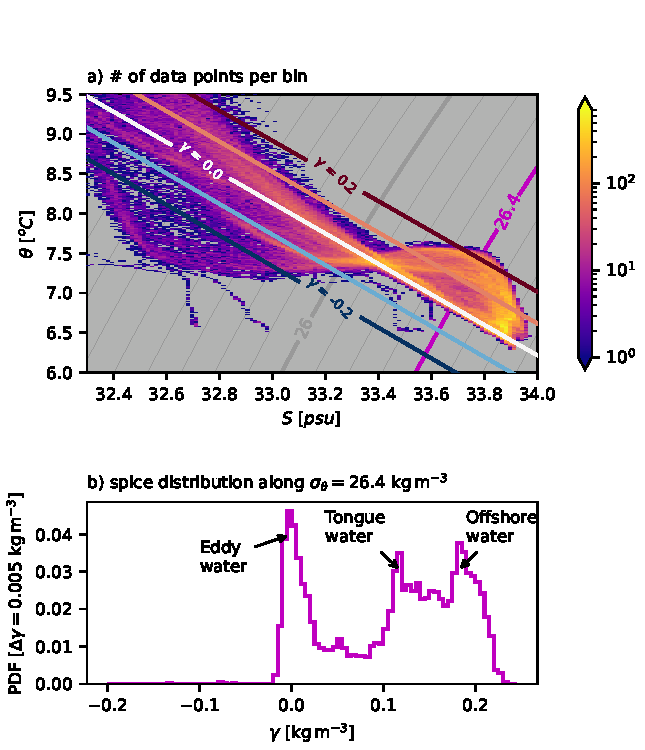
\includegraphics[width=3.5in]{TSdensSpice.pdf}
    \caption{\DIFaddbeginFL \DIFaddFL{a) }\DIFaddendFL Binned sample density of salinity and potential temperature from the cruise, with a logarithmic color scale.  Grey contours are potential density relative to the surface at intervals of $0.1\ \mathrm{kg\,m^{-3}}$; the magenta contour is the $26.4\ \mathrm{kg\,m^{-3}}$ isopycnal.  Colored contours are spice anomaly, $\gamma$, relative to the white line labeled $\gamma=0.0$.  \DIFaddbeginFL \DIFaddFL{b) Distribution of spice, $\gamma$ along the $26.4\ \mathrm{kg\,m^{-3}}$ isopycnal.
    }\DIFaddendFL \label{fig:TSdensSpice}}
  \end{center}
\end{figure*}

In synthetic cross sections of spice anomaly, the \Eddy\ is clearly identifiable as having low spice anomaly ($\gamma \approx 0\ \mathrm{kg\,m^{-3}}$, \fref{fig:CrossSectionsSpice}c, d). \DIFdelbegin \DIFdel{This signature of well-mixed }\DIFdelend \DIFaddbegin \DIFadd{These lines are made with a two-dimensional interpolation where MVP casts at a given depth are given a Gaussian weight $w = e^{-(r/r_0)^2}$, where $r$ is the distance from the line and $r_0 = 1.5\ \mathrm{km}$.  Note that the section at   The low-spice anomaly }\DIFaddend water extends from the seafloor to approximately 30 m depth, onshore of $X \approx 0\ \mathrm{km}$.  Despite lying along a mixing line, the \Eddy\ water is still stratified.  The high-spice water ($\gamma \approx 0.2\ \mathrm{kg\,m^{-3}}$) is found offshore of the \Eddy\ water, on the other side of a sharp $\theta-S$ compensated front. This front is even sharper in individual sections than in these composite sections (see \fref{sec:frontsurvey}).

In contrast, the third population of partially mixed water between the \Eddy\ and offshore water (\fref{fig:TSdensSpice}) is all found poleward of the \Eddy\ region (\fref{fig:CrossSectionsSpice}a, b) as water with a weaker spice anomaly ($\gamma \approx 0.1\ \mathrm{kg\,m^{-3}}$, pink colors).  This water is not as warm as offshore water, indicating some mixing with offshore water has taken place.  Of note is that this intermediate water mass appears completely absent in the sections further equatorward (\fref{fig:CrossSectionsSpice}c, d), indicating that it is either mixed away or that it is advected elsewhere; we argue below that it is advected offshore in a large-scale tongue.


\begin{figure*}[htbp]
  \begin{center}
    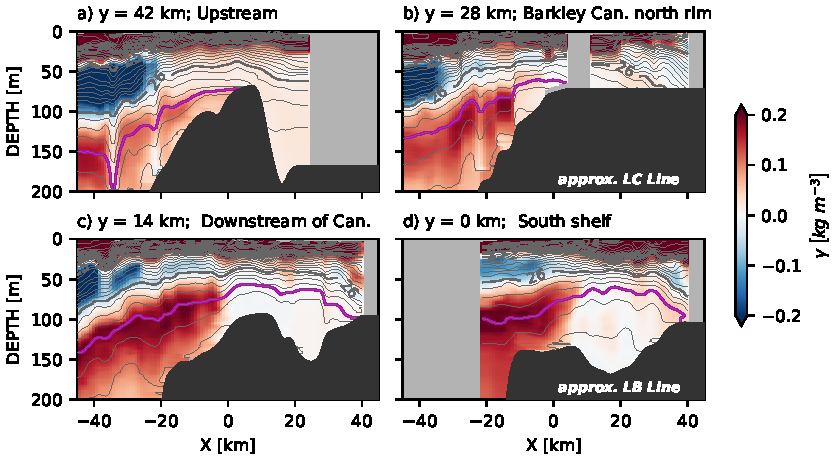
\includegraphics[width=6.2in]{CrossSectionsSpice}
    \caption{Synthetic sections of spice anomaly from the MVP data, projected along four lines from poleward (upstream of coastal current) a) to equatorward (downstream); the lines are shown in \fref{fig:LocMapBoth}\DIFdelbeginFL \DIFdelFL{b}\DIFdelendFL \DIFaddbeginFL \DIFaddFL{a}\DIFaddendFL ).    Isopycnals are contoured every $\sigma_{\theta} = 0.2\,\mathrm{kg\,m^{-3}}$ , with the $\sigma_{\theta} = 26.4\,\mathrm{kg\,m^{-3}}$ isopycnal highlighted in magenta.  Colors are spice anomaly as defined in \fref{fig:TSdensSpice}. "BC" in panel (c) refers to Barkley Canyon. \DIFaddbeginFL \DIFaddFL{Note that b) is along LC line (}\fref{fig:LaPerouse2013Ctd}\DIFaddFL{a--c,g--i), and d) is along the LB line (}\fref{fig:LaPerouse2013Ctd}\DIFaddFL{d--f,j--l).
      }\DIFaddendFL \label{fig:CrossSectionsSpice} }
  \end{center}
\end{figure*}

Oxygen saturation sections show that the deep water in the  \Eddy\ has very low oxygen saturation (\fref{fig:CrossSectionsO2}c, d) compared to surrounding water (though again, we caution against the quality of these saturation values from such a fast profiling instrument with a slow response time).  More oxygenated water is found offshore, and the oxygen deficit is not as strong in the poleward sections (\fref{fig:CrossSectionsO2}a, b).  The T/S compensated front also shows an abrupt transition from the \Eddy\ water and the offshore. Note the excellent correlation between oxygen saturation and spice anomaly in \fref{fig:CrossSectionsSpice}.

\begin{figure*}[htbp]
  \begin{center}
    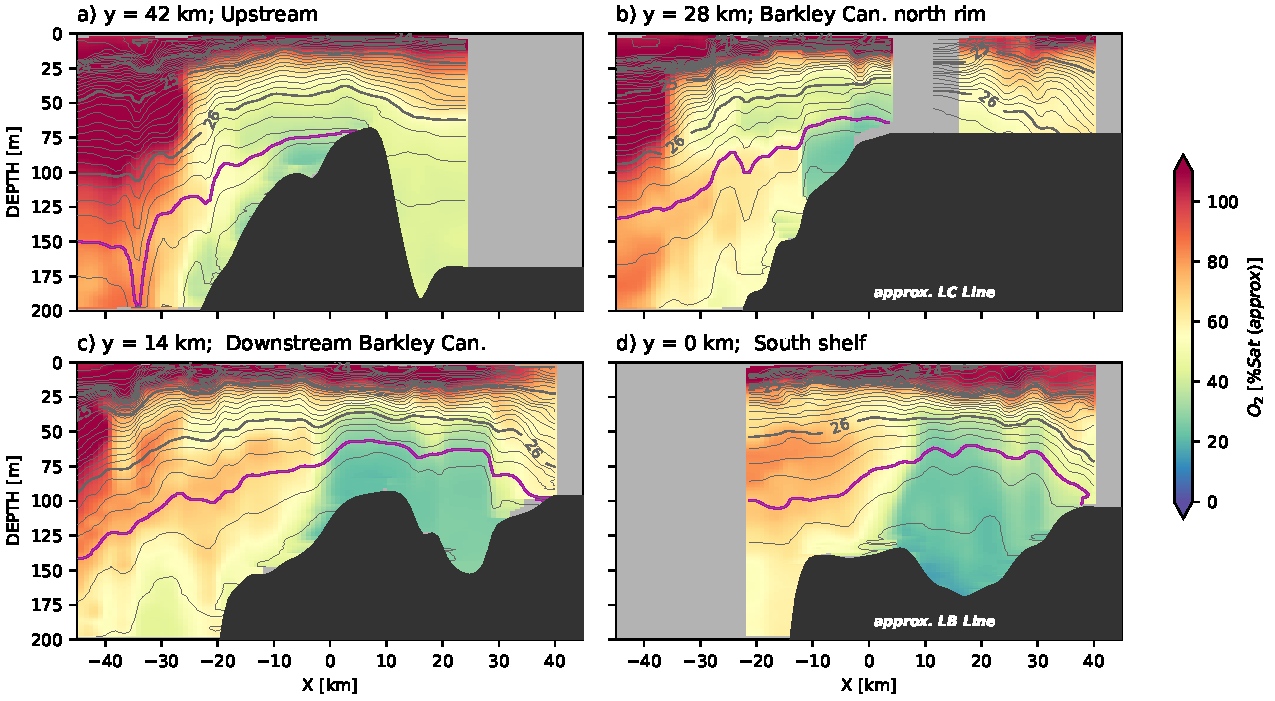
\includegraphics[width=6.2in]{CrossSectionsO2}
    \caption{As in \fref{fig:CrossSectionsSpice}, for oxygen approximate saturation.
      \label{fig:CrossSectionsO2} }
  \end{center}
\end{figure*}

The spatial patterns are very clear when considering a map view of properties along the $\sigma_{\theta} = 26.4\,\mathrm{kg\,m^{-3}}$ isopycnal (\fref{fig:SpiceO2264}).  There is a region onshore of the south tip of La Perouse Bank (approximately \DIFdelbegin \DIFdel{44.5}\DIFdelend \DIFaddbegin \DIFadd{48.5}\DIFaddend \textdegree N, 125.75\textdegree W), that consists of water that is found along the mixing line (spice anomaly $\gamma \approx 0\ \mathrm{kg\,m^{-3}}$) that also has low oxygen saturation.  Offshore of this region is water that is very warm and salty in comparison ($\gamma > 0.15 \mathrm{kg\,m^{-3}}$), and relatively high in oxygen (saturations of approximately 60\%).  The \DIFdelbegin \DIFdel{region }\DIFdelend \DIFaddbegin \DIFadd{transition }\DIFaddend between these two water masses is very abrupt, and  stretches from La Perouse Bank to a shallow bank just above the Juan de Fuca \DIFdelbegin \DIFdel{canyon }\DIFdelend \DIFaddbegin \DIFadd{Canyon }\DIFaddend (48.3\textdegree N and 125.4\textdegree W).

Poleward of La Perouse bank and Barkley Canyon, the water along the shelf has the weaker spice anomaly characteristic of the third water mass ($\gamma \approx 0.1\,\mathrm{kg\,m^{-3}}$, light pink colors).  This water is also somewhat lower in oxygen than water from offshore, though not as depleted as the water in the \Eddy.  \DIFdelbegin \DIFdel{This }\DIFdelend \DIFaddbegin \DIFadd{The }\DIFaddend water appears to be pushed offshore just upstream of Barkley Canyon and replaced on the shelf by the warmer (high spice) offshore water.

\DIFaddbegin \DIFadd{The correspondence between low oxygen water and water on the mixing line that defines $\gamma \approx 0\ \mathrm{kg\,m^{-3}}$ is quite strong (}\fref{fig:SpiceO2264}\DIFadd{c).  Eddy water is onshore (more red colors), low in oxygen, and along the mixing line.   Offshore water is high in oxygen and has a high spice anomaly.  Water that is found poleward on the shelf is still relatively high oxygen, but of intermediate spice $\gamma \approx 0.125\ \mathrm{kg\,m^{-3}}$.
}

\DIFaddend \begin{figure*}[htbp]
  \begin{center}
    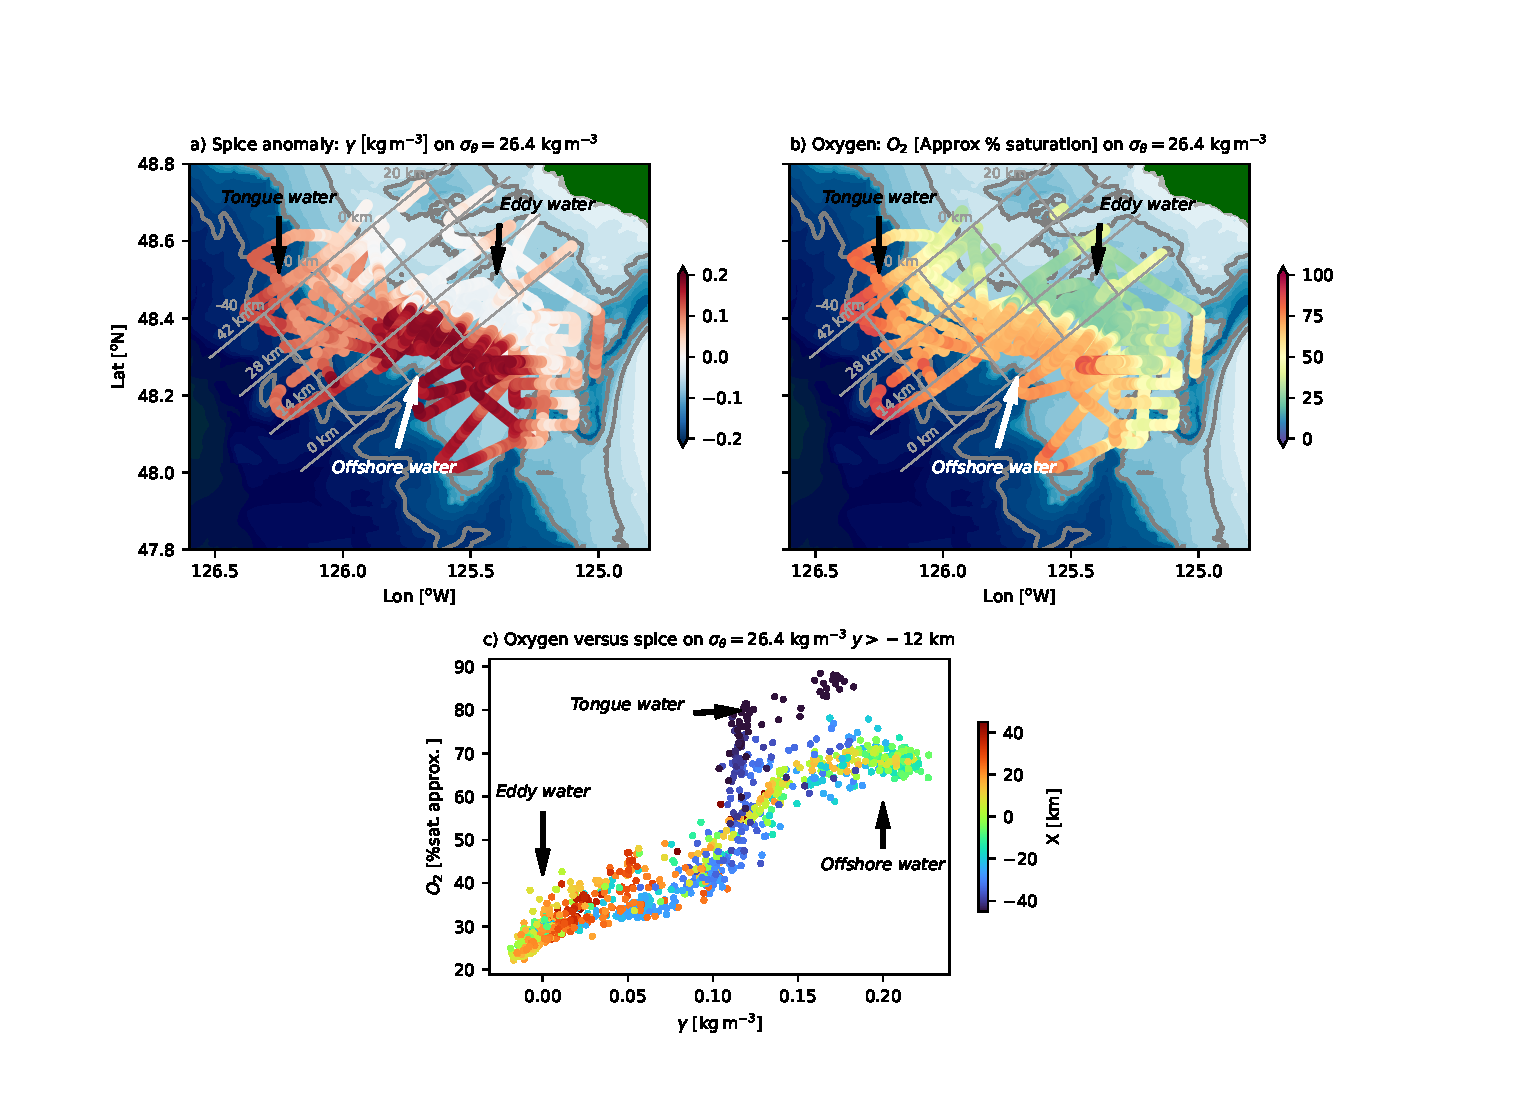
\includegraphics[width=6.2in]{SpiceO2264}
    \caption{Spatial overview of a) the spice anomaly, and b) oxygen saturation on the $\sigma_{\theta} = 26.4\ \mathrm{kg\,m^{-3}}$ isopycnal.  Grey cross-slope lines are cross sections indicated in \fref{fig:CrossSectionsSpice}.  Along-slope grey lines are every 20 km in the cross-slope direction, with $X=0\ \mathrm{km}$ near the 100-m isobath at the north end of the observation area. \DIFaddbeginFL \DIFaddFL{c) distribution of oxygen as a function of spice anomaly and $\sigma_{\theta} = 26.4\ \mathrm{kg\,m^{-3}}$, colored by x-coordinate. Data from the Juan de Fuca Canyon region ($y<-12\ \mathrm{km}$) is not shown.
   }\DIFaddendFL \label{fig:SpiceO2264}
    }
  \end{center}
\end{figure*}

\subsubsection{Spur Canyon}
%%%%%%%%%%%%%%%%%%%%%%%%%%%%%%%%%%%%%%%%

The Spur Canyon leading from the Strait of Juan de Fuca has been implicated in allowing dense water to be upwelled into the \Eddy \DIFaddbegin \DIFadd{\mbox{%DIFAUXCMD
\cite{mackasetal87,weaverhsieh87}}\hskip0pt%DIFAUXCMD
}\DIFaddend .  The sea surface is low in the middle of the \Eddy, so it has been hypothesized that water moves up the Spur Canyon due to ageostrophic motion \cite{weaverhsieh87,freelanddenman82}.  \DIFdelbegin \DIFdel{This }\DIFdelend \DIFaddbegin \DIFadd{It }\DIFaddend is difficult to infer \DIFaddbegin \DIFadd{flow up the Spur Canyon }\DIFaddend from the observations collected here.  Three transects up the canyon indicate that deep isopycnals slope up into the canyon (\fref{fig:CanyonPropertiesSpice}, to approximately 30 km).  Continuing across the \Eddy, isopycnals are largely flat until they intersect the Vancouver Island Coastal Current (\DIFdelbegin \DIFdel{$80\ \mathrm{km}$}\DIFdelend \DIFaddbegin \DIFadd{$X_{canyon} = 80\ \mathrm{km}$}\DIFaddend ).  The deeper isopycnals are not found in the deeper basin northeast of La Perouse \DIFdelbegin \DIFdel{bank }\DIFdelend \DIFaddbegin \DIFadd{Bank }\DIFaddend ($70\ \mathrm{km}$),  thus the bank is a natural poleward boundary of the \Eddy.

\begin{figure*}[htbp]
  \begin{center}
    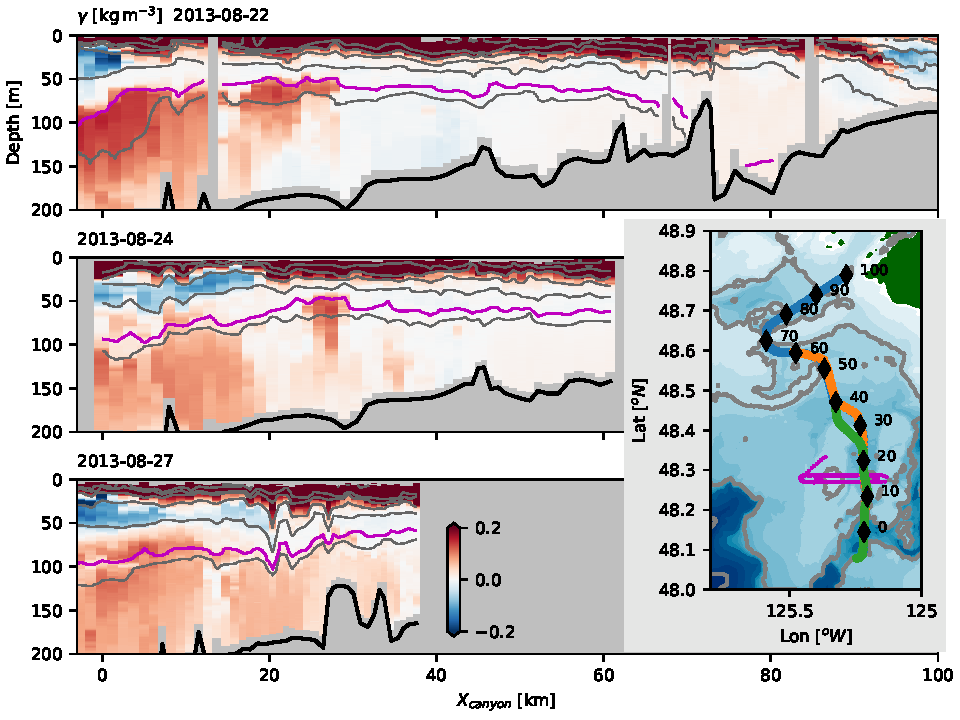
\includegraphics[width=6.2in]{CanyonPropertiesSpice}
    \caption{Spice anomaly surveys up the Spur Canyon, where \DIFdelbeginFL \DIFdelFL{$X$ }\DIFdelendFL \DIFaddbeginFL \DIFaddFL{$X_{canyon}$ }\DIFaddendFL is along-canyon as defined in the map.  Grey isopycnals are contoured every $0.5\,\mathrm{kg\,m^{-3}}$, and the $26.4\,\mathrm{kg\,m^{-3}}$ isopycnal is shown in magenta.  The seafloor is indicated with the thick black line.  Map (lower right) shows the path taken during each survey in chronological order (blue, orange, and green).  Magenta line is path taken during a cross-canyon survey (\fref{fig:HydraulicsCanyon}).
      \label{fig:CanyonPropertiesSpice} }
  \end{center}
\end{figure*}

Spice anomaly along the canyon indicates a transition from offshore water to \Eddy\ water.  Oxygen saturation behaves in a similar manner, though some of the incoming water has slightly lower oxygen than water inside the \Eddy\ (not shown).  Based on these sections, it is difficult to infer water motion up the canyon.

Much of the modified water in the Spur Canyon appears to come from the shelf to the west, but heavily modified by tidal mixing. A repeat tidal survey over the bank on the west side of the canyon shows a strong hydraulic response during onshore flow (17:58--21:00, \fref{fig:HydraulicsCanyon}).  Dense water passes from the offshore side into the canyon, and plunges down the side wall before rebounding downstream.  Note that the tide here is largely diurnal, so this onslope flow only occurs once a day.  Given the stratification of $N\approx 6\times10^{-3} \ \mathrm{rad\,s^{-1}}$ and an overturning scale of 50 m, we might expect dissipation rates reaching $\epsilon \sim L^2N^{3} \approx 5\times10^{-4}\ \mathrm{m^2\,s^{-3}}$, which is three orders of magnitude higher than dissipation observed on the shelf west of this location by \citeA{deweycrawford88}.  This estimate of turbulence dissipation rate implies a diapycnal diffusivity of \DIFdelbegin \DIFdel{$\kappa = \gamma \epsilon / N^2 \approx 1\ \mathrm{m^2\,s^{-1}}$}\DIFdelend \DIFaddbegin \DIFadd{$\kappa = \gamma \epsilon / N^2 \approx 0.5$ -- $5\ \mathrm{m^2\,s^{-1}}$}\DIFaddend , assuming a mixing efficiency of $\gamma=0.2$. Water spills over from the offshore front into the canyon during the onshore tide.  This water is rapidly mixed with surrounding water such that its strong offshore spice values are attenuated.

\begin{figure*}[htbp]
  \begin{center}
    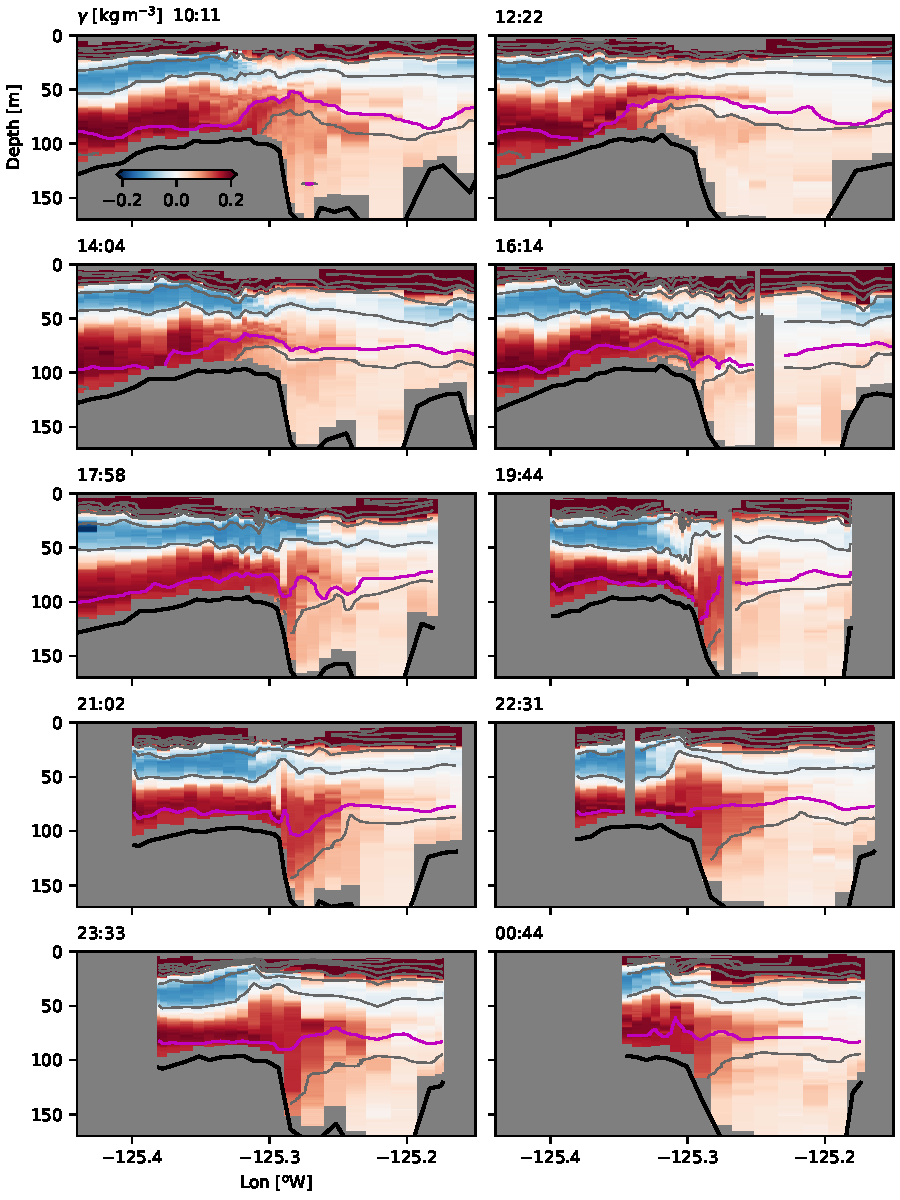
\includegraphics[width=4in]{HydraulicsCanyon}
    \caption{Spice anomaly observed in repeated, tide-resolving survey across the Spur Canyon, time is indicated in the upper left of each plot (29 August, 2013).   Location of survey shown in \fref{fig:CanyonPropertiesSpice} as a magenta line.
      \label{fig:HydraulicsCanyon}
    }
  \end{center}
\end{figure*}

The turbulence found on the canyon rim makes it ambiguous if there is water moving up the canyon or not.  There is a general tendency along the canyon for higher spice water to be found offshore (\fref{fig:CanyonPropertiesSpice}) but it seems likely that the source of the higher spice water is from over the bank rather than water being advected up the canyon.  \DIFdelbegin \DIFdel{This }\DIFdelend \DIFaddbegin \DIFadd{The }\DIFaddend tidally driven flow over the bank is the most significant source of high-spice offshore water into the \DIFdelbegin \DIFdel{eddy }\DIFdelend \DIFaddbegin \Eddy\DIFadd{\ }\DIFaddend region identified during our surveys.

\subsubsection{Frontal survey}
\label{sec:frontsurvey}
%%%%%%%%%%%%%%%%%%%%%%%%%%%%%%%%%%%%%%%%

A systematic survey through the front between the offshore water and the \Eddy\ water demonstrates the sharpness and persistence of this front (\fref{fig:Frontsurvey}), suggesting that it has limited exchange with the offshore region.

The survey started close to shore, and passed through the Vancouver Island Coastal Current (along-track 0-10 km).  The coastal current forms a buoyant \DIFdelbegin \DIFdel{front}\DIFdelend \DIFaddbegin \DIFadd{current}\DIFaddend , and is fresher and colder than water at the same density.  \DIFdelbegin \DIFdel{This front }\DIFdelend \DIFaddbegin \DIFadd{The front with the coastal water }\DIFaddend is relatively thick, greater than 20 km wide, and has \DIFaddbegin \DIFadd{entrained }\DIFaddend partially mixed water \DIFaddbegin \DIFadd{down }\DIFaddend from the surface to the foot of the front ($\gamma\approx0.1$).

Offshore of this coastal current, measurements were collected crossing the front between the offshore water and the \Eddy\ water 10 times, showing its evolution following the along-shore equatorward flow.  First, as noted in the composite sections, isopycnals slope up from offshore onto the shelf.  In the first crossing, the front is very sharp, (along-track distance $50\ \mathrm{km}$) though two small tendrils \DIFaddbegin \DIFadd{of higher spice water }\DIFaddend can be seen separating from the front on the inshore side.  Similar tendrils are found on the second crossing, perhaps a bit more separated from the front ($\approx 80\ \mathrm{km}$), and on the third crossing ($\approx 95\ \mathrm{km}$).  These tendrils are made of up partially mixed water.  The subsequent passes have more of this partially mixed water, such that the partially mixed front is up to 5-km wide by the fifth pass ($\approx 150\ \mathrm{km}$).  However, the deeper isopycnals retain a sharp front, and indeed the front appears sharp again by the seventh pass at all depths ($\approx 200\ \mathrm{km}$).

There is evidence of some warmer water swirling into \DIFdelbegin \DIFdel{Eddy}\DIFdelend \DIFaddbegin \Eddy\DIFaddend , particularly along isopycnals deeper than $26.4\,\mathrm{kg\,m^{-3}}$.  Regions of warmer (and more oxygenated) water are found in tendrils at these depths (e.g.\ \DIFdelbegin \DIFdel{$\approx\,170\ \mathrm{km}$ }\DIFdelend \DIFaddbegin \DIFadd{$\approx 170\ \mathrm{km}$ }\DIFaddend and $\approx 185\,\mathrm{km}$).  The overall effect is similar to what was seen in the Gulf Stream with similar observations \cite{klymaketal16}; there are two quite distinct water masses, the \DIFdelbegin \DIFdel{Eddy }\DIFdelend \DIFaddbegin \Eddy\DIFadd{\ }\DIFaddend water and the offshore water, as seen in the $\theta$--$S$ plot (\fref{fig:Frontsurvey}c) with only a small population of samples between these two.  \DIFdelbegin \DIFdel{This distribution of }\DIFdelend \DIFaddbegin \DIFadd{These distinct }\DIFaddend $\theta$--$S$ properties \DIFdelbegin \DIFdel{is }\DIFdelend \DIFaddbegin \DIFadd{are }\DIFaddend indicative of substantial isopycnal and vertical mixing, but even these populations are relatively cut off from the main water masses, indicating that they are well-mixed on their own, in short episodic events.  Regardless, this front is very sharp given that it has no density signature, indicating that there is not strong advection from offshore into the \Eddy\ region.

\begin{figure*}[htbp]
  \begin{center}
    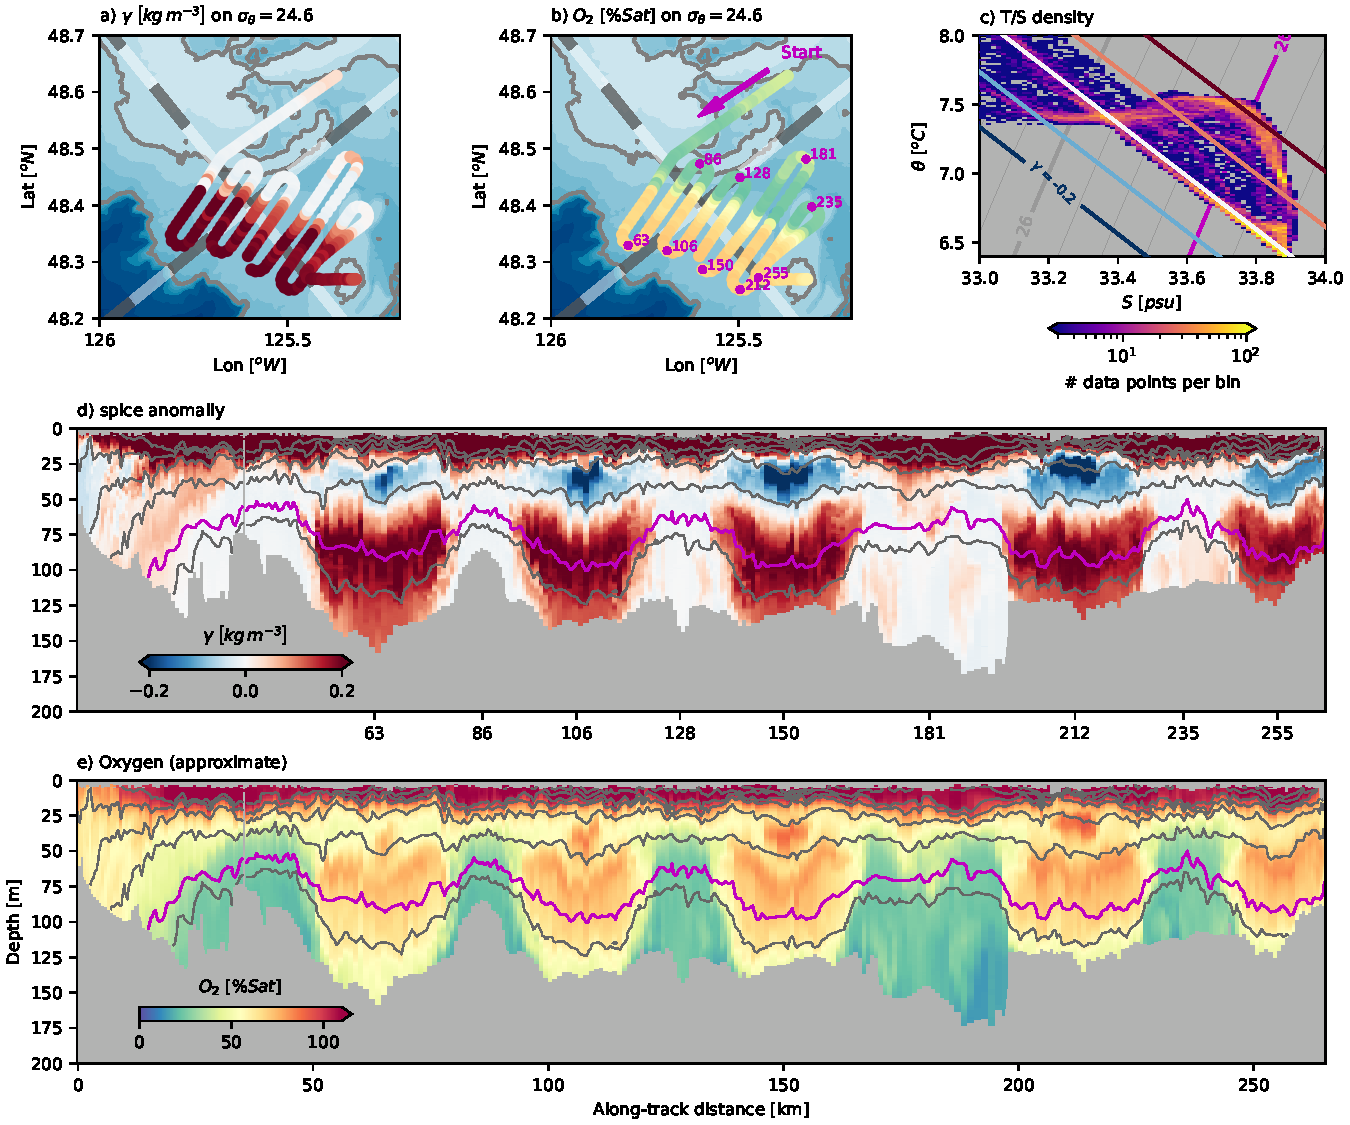
\includegraphics[width=6.2in]{Frontsurvey}
    \caption{Data from the \DIFdelbeginFL \DIFdelFL{frontal }\DIFdelendFL \DIFaddbeginFL \DIFaddFL{offshore front }\DIFaddendFL survey  a) spice anomaly along $26.4\,\mathrm{kg\,m^{-3}}$.  Grey-white alternating lines are the coordinate system, with 10-km alternating shades.   b) oxygen saturation along $26.4\,\mathrm{kg\,m^{-3}}$; magenta dots correspond to \DIFaddbeginFL \DIFaddFL{turn locations as }\DIFaddendFL distance along-track. c) density of data points (logscale) in this section of data.  d) cross-section of spice anomaly along track.  Grey isopycnals are contoured every $0.5\,\mathrm{kg\,m^{-3}}$, and the $26.4\,\mathrm{kg\,m^{-3}}$ isopycnal is shown in magenta. \DIFaddbeginFL \DIFaddFL{Ticks are turn locations }\DIFaddendFL e) cross-section of oxygen saturation.
      \label{fig:Frontsurvey} }
  \end{center}
\end{figure*}

%%%%%%%%%%%%%%%%%%%%%%%%%%%%%%%%%%%%%%%%
\subsection{Separation of coastal water}
%%%%%%%%%%%%%%%%%%%%%%%%%%%%%%%%%%%%%%%%

Upstream of the the sharp front between the low-spice \Eddy\ and the high-spice offshore water is a substantial mass of intermediate-spice water along the shelf (compare \fref{fig:CrossSectionsSpice}a and c).   This intermediate spice water is moving equatorward along the shelf upstream of the \Eddy, but is pushed offshore just upstream of Barkley Canyon (\fref{fig:IsopycnalsDepth}\DIFaddbegin \DIFadd{d}\DIFaddend ).  There is a tongue of intermediate-spice water (\DIFdelbegin \DIFdel{$\gamma$ is }\DIFdelend \DIFaddbegin \DIFadd{$\gamma \approx 0.1\,\mathrm{kg\,m^{-3}}$, }\DIFaddend pink along $26.4\,\mathrm{kg\,m^{-3}}$) that separates from the shelf just west of 126\textdegree W. The surveys do not cross the full extent of the  tongue, but it is at least 30 km wide. It also appears to end at approximately 48.2\textdegree N.  This intermediate-spice water reaches from relatively shallow isopycnals to at least \DIFdelbegin \DIFdel{$26.6\,\mathrm{kg\,m^{-3}}$ }\DIFdelend \DIFaddbegin \DIFadd{$26.55\,\mathrm{kg\,m^{-3}}$ }\DIFaddend (\fref{fig:IsopycnalsDepth}\DIFdelbegin \DIFdel{, left panel}\DIFdelend \DIFaddbegin \DIFadd{h}\DIFaddend ).  Unfortunately, we cannot track the fate of this water mass because isopycnals tilt down offshore, below the depth limit of the MVP.   The \DIFdelbegin \DIFdel{$25.5\,\mathrm{kg\,m^{-3}}$ }\DIFdelend \DIFaddbegin \DIFadd{$25.8\,\mathrm{kg\,m^{-3}}$ }\DIFaddend isopycnal appears to have the tongue \DIFaddbegin \DIFadd{(}\fref{fig:IsopycnalsDepth}\DIFadd{a), but }\DIFaddend closer to the shelf than at $26.4\,\mathrm{kg\,m^{-3}}$, indicating strong three-dimensionality to this feature.

This separating tongue is embedded in the larger scale isopycnal tilt caused by the upwelling (\fref{fig:IsopycnalsDepth}, \DIFdelbegin \DIFdel{right panels}\DIFdelend \DIFaddbegin \DIFadd{c,f, and j}\DIFaddend ), so it is difficult to see dynamically what is driving this offshore push.  \DIFaddbegin \DIFadd{If the offshore motion were geostrophically balanced, we would expect the isopycnals to dome upwards from poleward towards Barkley Canyon, but if such doming is happening, it is weaker than variability from internal tides and synoptic unsteadiness. }\DIFaddend One possibility is that it is simple flow separation caused by the water not being able to make the sharp turn around La Perouse Bank\DIFaddbegin \DIFadd{, which would be an ageostrophic effect}\DIFaddend .  Whatever causes it, downstream of the separation, the water is replaced by offshore water with much higher spice values.  \DIFaddbegin \DIFadd{The high-spice water comes onto the shelf through much of the water column, so is not just being carried onshelf by near-bottom Ekman layer by wind driven upwelling.
}\DIFaddend 

\begin{figure*}[htbp]
  \begin{center}
    \includegraphics[width=6.2in]{IsopycnalsDepth}
    \caption{Isopycnal slices \DIFdelbeginFL \DIFdelFL{through }\DIFdelendFL \DIFaddbeginFL \DIFaddFL{of the MVP data }\DIFaddendFL showing the vertical structure of the water separating from the shelf, with the first row along $25.5 \,\mathrm{kg\,m^{-3}}$, second along $26.4\,\mathrm{kg\,m^{-3}}$, and the third at $26.6\,\mathrm{kg\,m^{-3}}$.  First column is the spice anomaly, second is oxygen saturation, and the last column is depth of each isopycnal.
      \label{fig:IsopycnalsDepth} }
  \end{center}
\end{figure*}

There is a clear surface expression of the separating tongue in satellite imagery (\fref{fig:SST}).  Water flowing equatorward along the shelf tends to be cooler than offshore water, likely due to mixing with the colder coming out of the Strait of Juan de Fuca. On August 25, there is a cold tongue of water separating from La Perouse \DIFdelbegin \DIFdel{bank}\DIFdelend \DIFaddbegin \DIFadd{Bank}\DIFaddend , crossing isobaths and pointing south at 125.8\textdegree W.   There is a cooler tendril streaming west at 48 N off the south end of this tongue.  This feature is not as well-developed in the previous image (Aug.\ 21) perhaps indicating that it is an evolving feature.  By 31 August, there is no surface expression of the feature, though small tendrils of cooler water can be seen separating from La Perouse Bank.  By 5 September, the water has significantly warmed, and the offshore anomaly does not appear to have a surface signature.

\begin{figure}
  \begin{center}
    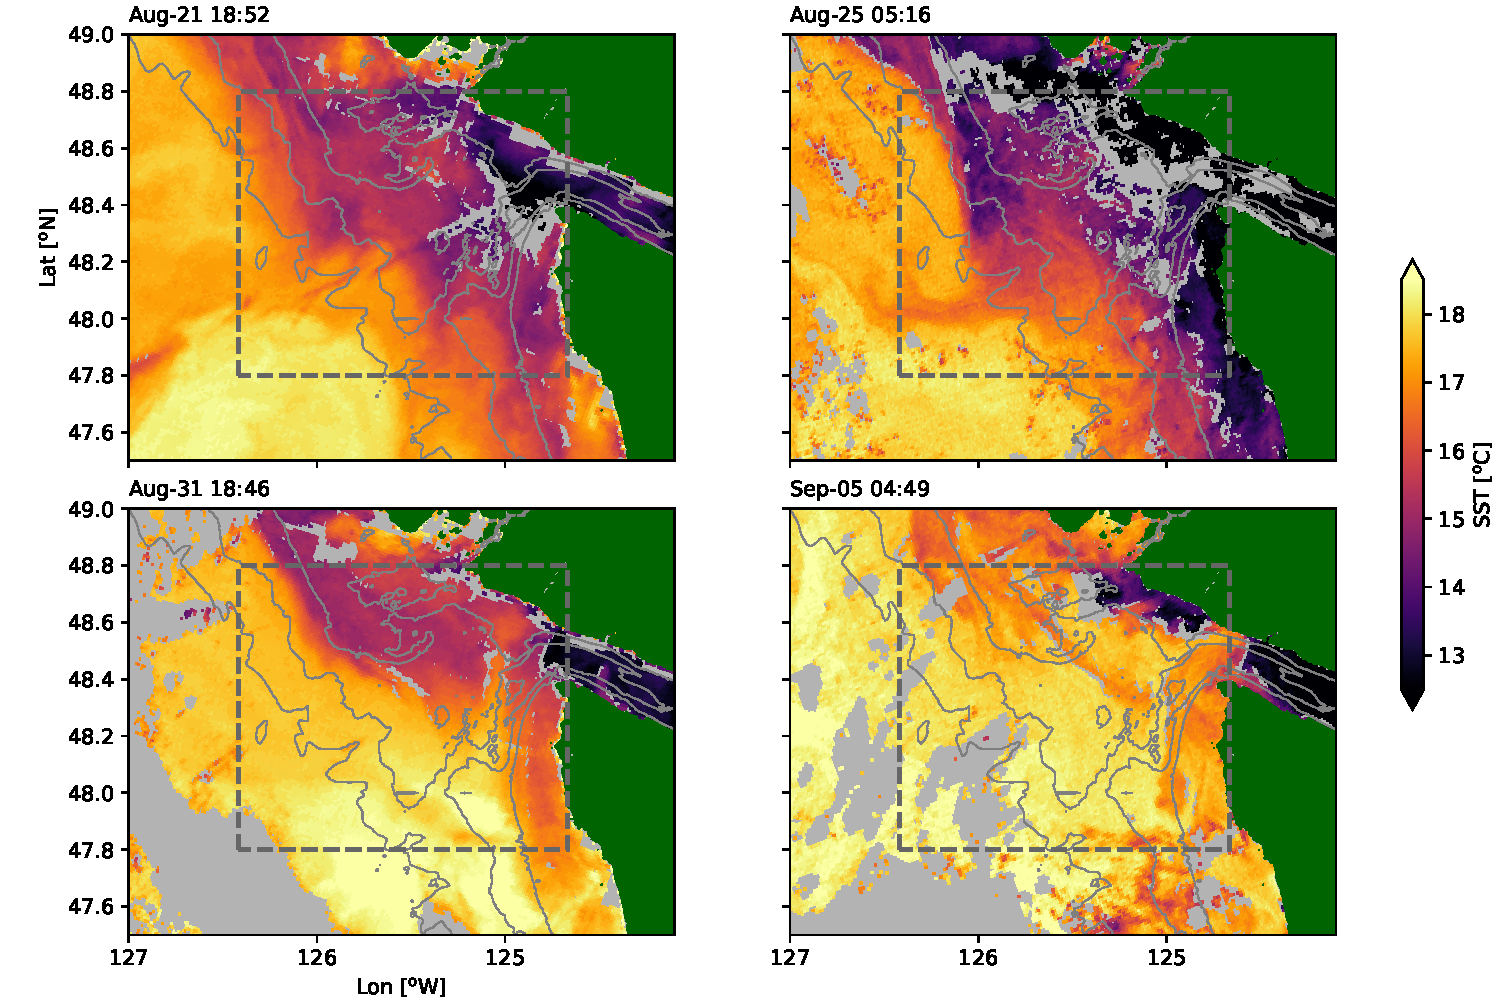
\includegraphics[width=6in]{SSTSnaps}
    \caption{Sea surface temperature snapshots from the observation period.  Grey areas are clouds; dashed gray line is the study area. Depths are contoured in thin gray lines at 200, 150 and 100 m. \cite{L2PMetopA}\label{fig:SST}}
  \end{center}
\end{figure}

Satellite-based surface chlorophyll estimates show the same feature (\fref{fig:ChlA}) \DIFdelbegin \DIFdel{demonstrating }\DIFdelend \DIFaddbegin \DIFadd{suggesting }\DIFaddend the advection of high chlorophyll to the west side of the \Eddy. They also show a relatively high-chlorophyll tendril to the west, again exiting the study region at approximately 48 degrees N.  The feature is relatively long-lived, on the order of one month.  Inspection of images before August 5 were too obscured by clouds or did not show this feature.  By September 6, we see the feature fading from the satellite image.  Note that this feature is centered 0.2 degrees of latitude south of tongue that we observe deeper in the water column, again indicating that there is depth-dependent structure in the feature.

\begin{figure*}[htbp]
  \begin{center}
    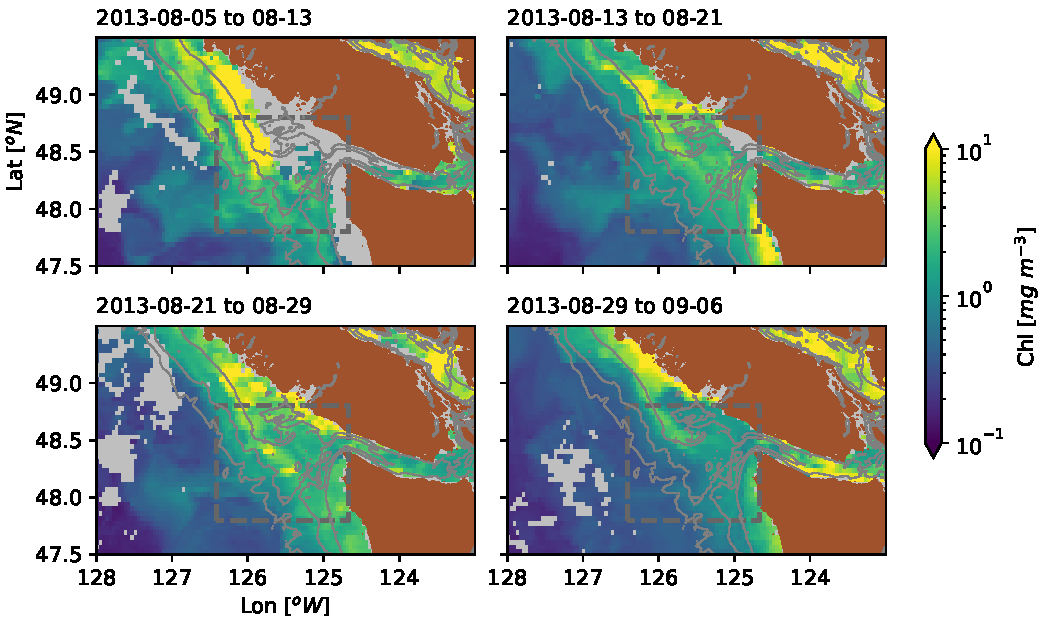
\includegraphics[width=6.2in]{ChlA}
    \caption{Surface chlorophyll density estimated from ocean color \cite{Huetal12,MODISChlL3} over 8-day windows in 4-km bins. Gray regions had too many clouds to compute averages.
      \label{fig:ChlA} }
  \end{center}
\end{figure*}


\section{Summary and Discussion}
\label{sec:Summary}

The intensive sampling discussed here has demonstrated a few important features of the South Vancouver Island Shelf.  The Juan de Fuca Eddy water is readily identified as falling along a mixing line in $\theta-S$ space, compared with offshore water that was warmer and saltier (high-spice anomaly).   There was not strong evidence of the \Eddy\ being supplied by water moving up the Spur Canyon during our observations, but the Spur Canyon was a site of hydraulic cross-canyon flows in which we infer significant mixing \DIFaddbegin \DIFadd{has occurred}\DIFaddend . There is a sharp and persistent temperature-salinity compensated front between offshore water and the partially mixed \Eddy\ water.  Finally, upstream of the \Eddy, water in the equatorward shelf current has intermediate spice anomaly, and is seen to separate from the shelf at the point of an abrupt bend in an underwater bank.  The water mass crosses isobaths and is ejected into the interior. This separation event can also be observed from satellite measurements of sea surface temperature and chlorophyll.  Thus the water that is offshore of the \Eddy\ appears to have been brought onto the shelf in exchange for the offshore ejection of shelf water via this tongue.

\subsection{Age and source of the \Eddy\ water}

The source of water and formation mechanism of the Juan de Fuca Eddy has received substantial attention, however, the observations of \Eddy\ waters being found along a tight mixing line in $\theta$--$S$ space has not previously been noted.  The deepest water in the \Eddy\ could originate along the $\theta$--$S$ line from approximately $5.5^\circ \mathrm{C}$ to $7.5^\circ \mathrm{C}$ (\fref{fig:LaPerouse2013TS}a), which in the open ocean spans depths from 420 m to 70 m.  \citeA{mackasetal87} attempted to determine the origin of the water by including oxygen as a third variable to resolve the ambiguous $\theta$--$S$ relation.  However, as \fref{fig:LaPerouse2013TS}b makes clear, oxygen does not appear to be a conserved property in the \Eddy, with concentrations up to $150 \ \mathrm{\mu mol\ kg^{1}}$ lower in the \Eddy\ than the water found offshore, and in a way that definitely cannot be the result of conservative mixing.  As a best guess, if the water in the deepest part of the \Eddy\ came from a vertical mixture of the water at $26.5\,\mathrm{kg\,m^{-3}}$ and an equal distance down in density space of $26.7\,\mathrm{kg\,m^{-3}}$, then the deepest water in the \Eddy\ may be coming from a depth of 250 m.  This is a typical upwelling depth for coastal flows, and may not require extra input up the Spur Canyon as posited by \citeA{freelanddenman82}.

We found little evidence of flow up the Spur Canyon or, if there is, then the mixing in the canyon is intense enough to remove the $\theta$--$S$ signature of offshore water within 20 km of the canyon mouth (\fref{fig:CanyonPropertiesSpice}).  We did find substantial evidence of mixing in the canyon, but the primary pathway of high-spice water into the canyon appears to be due to tidal flow over the banks on the west side (\fref{fig:HydraulicsCanyon}), rather than flow up the canyon.  However, it is worthy of note that upwelling winds had ceased at the point of these observations (\fref{fig:LaPeWind}), so the offshore surface pressure gradient may be reduced, leading to reduced ageostrophic upwelling in the canyon.  Whether the cessation of winds would also lead to a reduction of the low sea level height in the center of the \Eddy\ that may drive up-canyon flow is an open question.

There is evidence of aging of the water in the \Eddy\ between late spring and late summer (\fref{fig:LaPerouse2013Ctd}), with a reduction of oxygen in the \Eddy\ over this time span.  If we posited that the reduction was all in the same water, then the oxygen consumption rate over the time between the late-May and early September cruises would be on the order of $0.5\ \mathrm{\mu mol\, kg^{-1} d^{-1}}$.  This is on the low side of estimates of apparent oxygen utilization rates in continental upwelling systems, which are between $1$ and $5\  \mathrm{\mu mol\, kg^{-1} d^{-1}}$ \DIFdelbegin \DIFdel{\mbox{%DIFAUXCMD
\cite{dortchetal94}}\hskip0pt%DIFAUXCMD
}\DIFdelend \DIFaddbegin \DIFadd{\mbox{%DIFAUXCMD
\cite{dortchetal94,connollyetal10}}\hskip0pt%DIFAUXCMD
}\DIFaddend .   So it seems \DIFdelbegin \DIFdel{possible }\DIFdelend \DIFaddbegin \DIFadd{likely that }\DIFaddend the \Eddy\ \DIFdelbegin \DIFdel{had enough }\DIFdelend \DIFaddbegin \DIFadd{has }\DIFaddend exchange with the surrounding water\DIFdelbegin \DIFdel{for the residence time to have been less than the full time period from late May to September}\DIFdelend .  Note that during the May cruise, the water in the \Eddy\ is slightly cooler than the mixing line, and during the September cruise is slightly warmer than the mixing line, \DIFdelbegin \DIFdel{so }\DIFdelend \DIFaddbegin \DIFadd{further evidence that }\DIFaddend the water in the \Eddy\ is evolving seasonally \DIFdelbegin \DIFdel{, and probably affected by the water temperature in the }\DIFdelend \DIFaddbegin \DIFadd{(}\fref{fig:LaPerouse2013Ctd}\DIFadd{e,k).  This is consistent with findings on the Oregon shelf where physical processes are thought to account for 55-70\% of changes in dissolved oxygen concentrations \mbox{%DIFAUXCMD
\cite{adamsetal13}}\hskip0pt%DIFAUXCMD
.  Definitively identifying the exchange mechanisms into the }\Eddy\DIFadd{\ is challenging from this data set.  The offshore front does not appear to have much exchange, however as noted above there does appear to be strong tidal flows and mixing over the submarine banks that can transport more oxygenated water into the }\Eddy\DIFadd{.  Further, the }\DIFaddend Vancouver Island Coastal Current \DIFdelbegin \DIFdel{and the amount of water getting through the onshore front}\DIFdelend \DIFaddbegin \DIFadd{is oxygen-rich and has a much less sharp front than the offshore front (}\fref{fig:Frontsurvey}\DIFadd{), and is a likely source of oxygen to the }\Eddy\DIFaddend .

The water is  mixed enough in the \Eddy\ that it falls along a mixing line,
though it remains vertically stratified. The amount of homogenization is such
that either the mixing is very strong, or the water is retained in the \Eddy\
for a long time.  The amount of turbulence required to homogenize 100 m of
water over 90 days is $\kappa \approx 10^{-3}\ \mathrm{m^2\,s^{-1}}$.  Given
that the diffusivity implied in the cross-channel surveys was on the order of
\DIFdelbegin \DIFdel{$\kappa_{\rho} = 10 \ \mathrm{m^2\,s^{-1}}$}\DIFdelend \DIFaddbegin \DIFadd{$\kappa_{\rho} = 0.5$--$5\ \mathrm{m^2\,s^{-1}}$}\DIFaddend , this number is not outrageous
if we think that such high dissipation is found in \DIFdelbegin \DIFdel{$10^{-4}$ }\DIFdelend \DIFaddbegin \DIFadd{0.2--0.02\% }\DIFaddend of the water
column. We can more carefully quantify this by considering a synthetic profile
or temperature and salinity based on an offshore profile, extrapolated from the
bottom of the 200-m cast to 250 m, assuming that the temperature and salinity
at 250 m are $6.2\ \mathrm{[^oC]}$ and $34\ \mathrm{psu}$ respectively
(\fref{fig:TSExercise}).  Water at the offshore station was warmer than
onshore, so the profile was also linearly interpolated to a surface value of
($12\ \mathrm{^oC}$, $31.6\ \mathrm{psu}$).  The profile was then linearly
compressed into a depth range of 150 m representative of the shelf depth in the
dense pool, and subjected to mixing with a constant diffusivity of $\kappa =
10^{-3}\ \mathrm{m^2\,s^{-1}}$, with the surface and bottom values pinned under
the assumption that the near-bottom source and surface waters are replenished
from a large reservoir.  \DIFdelbegin \DIFdel{Similar to the naive scaling}\DIFdelend \DIFaddbegin \DIFadd{In this calculation}\DIFaddend , the T-S relationship does not
approach a straight line until after approximately 60-100 days, or until the
mixing affects a vertical length scale of \DIFdelbegin \DIFdel{$\lambda = \left(\tau \kappa\right)^{1/2}$ that is greater than $\approx 70\,\mathrm{m}$}\DIFdelend \DIFaddbegin \DIFadd{$\lambda = \left(\tau
\kappa\right)^{1/2} \gtrsim 70\,\mathrm{m}$}\DIFaddend .


\begin{figure*}[htbp]
  \begin{center}
    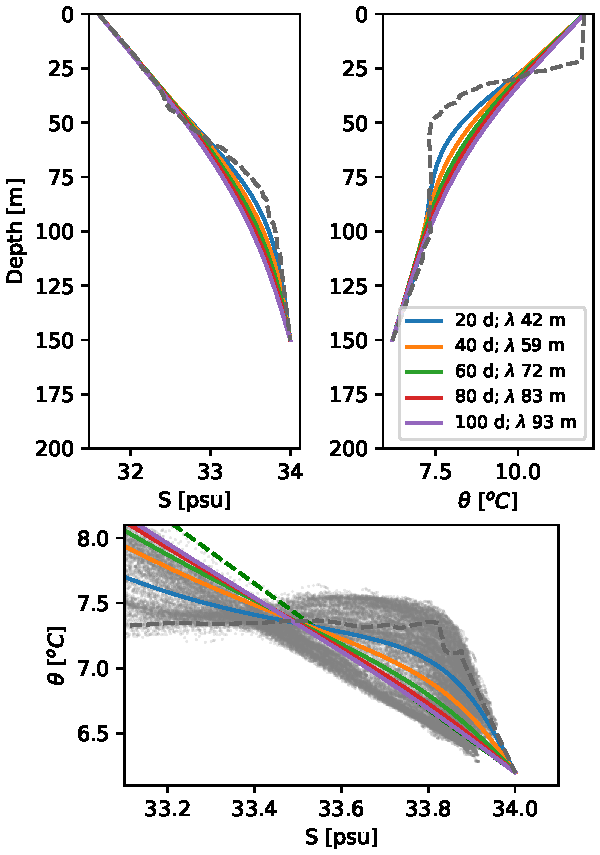
\includegraphics[width=4in]{TSExercise}
    \caption{Mixing model assuming constant eddy diffusivity of $\kappa = 10^{-3}\ \mathrm{m^2\,s^{-1}}$ acting on an offshore temperature and salinity profiles compressed from 250 thick to 150 m thick (grey dashed lines).  Profiles are pinned to the deep $\theta-S$ value at ($34\ \mathrm{psu}$, $6.2\ \mathrm{^oC}$), and a shallow one at ($31.6\ \mathrm{psu}$, $12\ \mathrm{^oC}$).  The green dashed line is the mixing line defined in the text.
      \label{fig:TSExercise} }
  \end{center}
\end{figure*}

\DIFaddbegin \DIFadd{Combined with the oxygen observations, the implication is that the water in the }\Eddy\DIFadd{\ likely experiences exchange with the outside water, but at a very modest rate.  In terms of a volume flux, we might estimate the }\Eddy\DIFadd{\ area as $900\ \mathrm{km^2}$, over 100 m depth, so that 100-d residence time corresponds to a transport of $10^{4}\ \mathrm{m^3s^{-1}}$, which is remarkably weak for the transport in and out of such a large area.
}

\DIFaddend The sharpness of the front with the \Eddy\ and the offshore water is
intriguing.  It was persistent for the duration of our detailed survey
(\fref{fig:SpiceO2264}), and, so far as we can tell with the limited resolution
of the hydrographic surveys, was present during the bracketing La Perouse
cruises. There is not any substantial bathymetry blocking the onshore incursion
of water at this location, so there must be a dynamic barrier.

Numerical simulations of this region reported by \cite{sahuetal22} using a NEMO
36th-degree regional model contained relatively rapid exchange between the deep
\Eddy\ water and the rest of the coastal ocean.  The region where the \Eddy\
resides has velocities equal or greater than other parts of the shelf, and
water has an approximate residence time of less than 20 days.  The \Eddy\ water
in the model does develop a distinct $\theta$--$S$ signature, but not along a
sharp mixing line as observed.  It also has a front with the offshore water,
but the front is substantially wider than that observed here.  \DIFaddbegin \DIFadd{Overall it seems
that the model sees stronger cross-shelf advection than are apparent in these
observations, though the reason for this will require further study.
}\DIFaddend 

Overall, it would be an improvement to our understanding of the \Eddy\ if we
could sample the shelf more persistently.  The \Eddy\ was already well-formed
by the May La Perouse cruise, and seems to evolve slowly during that time.
Capturing its formation, presumably earlier in the spring, as well as its
evolution through the year, would be valuable in understanding retention and
exchange on this productive part of the shelf.

\subsection{Offshore exchange of shelf water}

The displacement of shelf water from La Perouse Bank is a dramatic departure from geostrophically balanced isobath-following flow.  Eddies have been known to separate from irregular coastal topography, both at the surface \cite{barthetal00} and deeper in the water column \cite{pellandetal13}.   It has been recognized that instabilities lead to exchange between the open ocean and the shelf at this location \cite{ikedaemery84, ikedaemery84}.   However, observations of the wholesale replacement of shelf water by a new water mass from offshore are \DIFaddbegin \DIFadd{relatively }\DIFaddend rare. In the  observations presented here, it is clear that water from as deep as 150 m is separating from the shelf and moving offshore (\fref{fig:SpiceO2264}, \fref{fig:IsopycnalsDepth}).

Satellite imagery shows that there is often exchange between coastal and deep waters along the Vancouver Island shelf (\fref{fig:SSTLateAug}).  Most years there are three of four large filaments from the shelf into the open ocean, many of them over 100 km long.  This length scale is longer than the 60 km inferred for this region by \citeA{ikedaetal84} using a four-layer instability analysis.  It is possible that there is spatial locking of these features, with a persistent separation at the north tip of Vancouver Island, and a strong tendency for one at 49.5 N. There is also evidence of separation events in most of the years, with 2011 being the only clear exception. General baroclinic instability of the upwelling front is a possible mechanism to drive offshore exchange \cite{ikedaetal84,durskiallen05}, but this tends to be shallow, with smaller-scale instabilities that will not extend as far into the interior ocean as observed here.  Rather it seems likely that the topographic change engendered by the sudden turn to the east of La Perouse \DIFdelbegin \DIFdel{bank }\DIFdelend \DIFaddbegin \DIFadd{Bank }\DIFaddend catalyses a larger scale instability at this location.  \DIFaddbegin \DIFadd{In California most of the cold filaments observed appear to be catalyzed by headlands and underwater topography \mbox{%DIFAUXCMD
\cite{strubetal91}}\hskip0pt%DIFAUXCMD
, though modelling studies find instabilities are possible even in two-dimensional flows \mbox{%DIFAUXCMD
\cite{pierceetal91}}\hskip0pt%DIFAUXCMD
.  }\DIFaddend \citeA{durskiallen05}, when modelling the Oregon shelf, found that including realistic shelf bathymetry catalyzed intermittent large-scale instabilities\DIFdelbegin \DIFdel{similar to the feature here}\DIFdelend , a finding that is deemed likely to apply at other coastal locations \cite{batteen97}.

Large-scale mixing between the shelf and open ocean has been evident since the satellite era.  Here we demonstrate that in the Vancouver Island shelf the flow is originating on the shelf and separating from the bathymetry and being injected into the interior.  A  similar observation was made by \citeA{barthetal00} downstream of Cape Blanco, Oregon, where the coastal current was observed to detach from the shelf in the lee of the cape and flow into the interior.  They hypothesized that as the current moved offshore, it deepened, stretching isopycnals and creating cyclonic relative vorticity that would tend to push the current back onshelf, but then it was caught in the undercurrent and stalled, being pushed offshore. It is also possible that coastally trapped waves in the region experience a hydraulic control, and these separation events are part of the response \cite{dalebarth01}.

\begin{figure*}[htbp]
  \begin{center}
    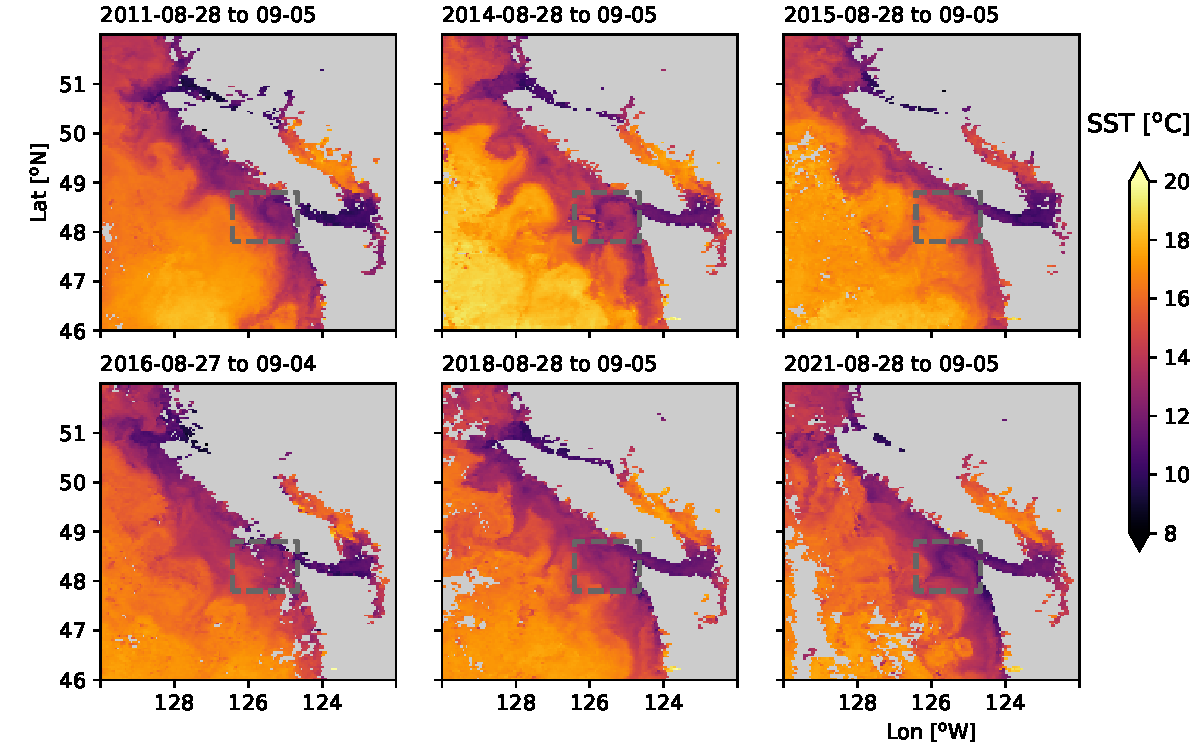
\includegraphics[width=6in]{SSTLateAug}
    \caption{
      Available late-August sea-surface temperature from 8-day composites, 2011 to 2021 \cite{MODISSST8d}; missing years had too much cloud cover or no satellite coverage.  \label{fig:SSTLateAug} }
  \end{center}
\end{figure*}

Regardless of the dynamics of the separation events, the offshore transport can be substantial.  If we assume the coastal current is approximately $0.1\ \mathrm{m\,s^{-1}}$ over 100 m in the vertical and 20 km in the horizontal, it represents 0.2 Sv of nutrient- and chlorophyll-rich shelf water transported offshore.  \DIFaddbegin \DIFadd{Sometimes the along-shelf currents are substantially larger than this \mbox{%DIFAUXCMD
\cite{thomsonkrassovski15} }\hskip0pt%DIFAUXCMD
reaching $0.4\ \mathrm{m\,s^{-1}}$.   }\DIFaddend Our observations are a \DIFdelbegin \DIFdel{finer detailed }\DIFdelend \DIFaddbegin \DIFadd{finer-detailed }\DIFaddend representation of the kind of cross-shore transports inferred by \citeA{mackasyelland99} from hydrographic surveys, and definitively show that this water can originate from the shelf from relatively deep depths and be transported offshore.  We do not have velocity measurements for the water that replaces it, but assuming that water also flows along-shelf, these separation events are associated with a large replacement of shelf water with offshore water at this location.  This emphasizes the importance of three dimensional observations and modeling of cross-shelf dynamics when thinking about physical and biological processes on the shelf.

\clearpage
%\section{Here Is Appendix Title}
% will show
% A: Here Is Appendix Title
%
%\appendix
%\section{Here is a sample appendix}

%%%%%%%%%%%%%%%%%%%%%%%%%%%%%%%%%%%%%%%%%%%%%%%%%%%%%%%%%%%%%%%%
%
% Optional Glossary, Notation or Acronym section goes here:
%
%%%%%%%%%%%%%%
% Glossary is only allowed in Reviews of Geophysics
%  \begin{glossary}
%  \term{Term}
%   Term Definition here
%  \term{Term}
%   Term Definition here
%  \term{Term}
%   Term Definition here
%  \end{glossary}

%
%%%%%%%%%%%%%%
% Acronyms
%   \begin{acronyms}
%   \acro{Acronym}
%   Definition here
%   \acro{EMOS}
%   Ensemble model output statistics
%   \acro{ECMWF}
%   Centre for Medium-Range Weather Forecasts
%   \end{acronyms}

%
%%%%%%%%%%%%%%
% Notation
%   \begin{notation}
%   \notation{$a+b$} Notation Definition here
%   \notation{$e=mc^2$}
%   Equation in German-born physicist Albert Einstein's theory of special
%  relativity that showed that the increased relativistic mass ($m$) of a
%  body comes from the energy of motion of the body—that is, its kinetic
%  energy ($E$)—divided by the speed of light squared ($c^2$).
%   \end{notation}




%%%%%%%%%%%%%%%%%%%%%%%%%%%%%%%%%%%%%%%%%%%%%%%%%%%%%%%%%%%%%%%%
%
%  ACKNOWLEDGMENTS
%
% The acknowledgments should list:
%
% 	All funding sources related to this work from all authors
%
% 	Any real or perceived financial conflicts of interests for any
%	author
%
% 	Other affiliations for any author that may be perceived as
% 	having a conflict of interest with respect to the results of this
% 	paper.
%
%   It is also the appropriate place to thank colleagues and other contributors.
%   AGU does not normally allow dedications.

%%%%%%%%%%%%%%%%%%%%%%%%%%%%%%%%%%%%%%%%%%%%%%%

\section*{Open Research}

Derived data files (1-m vertical binned CTD files) and analysis scripts are available at \url{https://ocean-physics.seos.uvic.ca/~jklymak/PW13DataAnalysis/}.  Raw CTD data is available on request.  Data was processed using a scientific python toolchain as listed at \url{https://ocean-physics.seos.uvic.ca/~jklymak/PW13DataAnalysis/environment.yml}; major
components include xarray \cite{xarray}, numpy \cite{numpy}, and Matplotlib \cite{Matplotlib36}, but those all leverage many smaller but vital projects.

\acknowledgments

Thank you to the officers and crew of the R/V Falkor and the Schmidt Foundation for funding the seagoing component of the cruise.  Thank you to Richard Dewey, Benjamin Schiefle, and Rowan Fox for efforts during the cruise\DIFaddbegin \DIFadd{.  Jack Barth and an anonymous reviewer provided valuable feedback on the manuscript}\DIFaddend .  Klymak was supported by NSERC Discovery grant RGPIN-2017-04050 and a Canadian Foundation for Innovation Leading Edge Fund grant 36109, Allen was supported by NSERC Discovery grant RGPIN-105694-11, and Waterman was supported by NSERC Discovery grant RGPIN-2020-05799.

\bibliography{main}

\end{document}
